\graphicspath{{chapt_dutch/}{intro/}{chapt2/}{chapt3/}{chapt4/}{chapt5/}{chapt6/}{chapt7/}{chapt8/}}

% Header
\renewcommand\evenpagerightmark{{\scshape\small Chapter 6}}
\renewcommand\oddpageleftmark{{\scshape\small Backgrounds Modelling and Data Driven Techniques for QCD estimation}}

\hyphenation{}

\chapter[Backgrounds Modelling and Data Driven Techniques for QCD estimation]%
{Backgrounds Modelling and Data Driven Techniques for QCD estimation}
\label{chapt:7}

\section{Backgrounds}
\label{sec:bkgs}

\section{Multijet Estimation}\label{sec:multijet}
One of the main background for semi-leptonic $t\bar{t}$ decays is the multijet QCD that has overwhelming cross section. Due to tight selection criteria, only a small fraction of these events mimics the semi-leptonic final state. This requires large simulation samples to have proper QCD modelling and enough statistics after the final selection that is not practical. We used data-driven technique to model our multijet QCD where we defined sideband regions in data that are enriched in QCD events. The distributions of the relevant kinematic variables for fitting taken directly from these data. The mass of $t\bar{t}$ and $cos\theta$* are used as normalization variables. In semi-leptonic decays of $t\bar{t}$, the multijet QCD background can mimic the signal via two main processes.
\begin{itemize}
\item Non-prompt and less isolated leptons from the decay of beauty and charm quarks. These are real leptons that gain significant $p_{T}$ from the mother b and c hadrons and have more activities in the vicinity. Lepton isolation cut suppresses these events.
\item Some hadrons didn't absorbed in the HCAL and make tracks in the muon system or jets with high electromagnetic fraction mimics electron signatures. They are treated as fake leptons.
\end{itemize}
Assuming that the kinematic properties of the multi jet events in selected phase space are independent of the lepton isolation in the event, we reversed the isolation cut to define the control region that is enriched of multijet events and less contamination from other processes. We use following selection criteria for lepton and event.
\begin{itemize}
\item Invert the lepton isolation cut to get enriched multijet QCD events and anti-isolation region is checked in three independent regions.
\item The rest of lepton selection are same as defined in section \ref{Sec:Reconstruction} for both muon and electron.
\item The definition of loose lepton is same as in section \ref{Sec:Reconstruction} but exclude from it the anti-isolated lepton.
\item Jets are cleaned against the isolated leptons.
\item The event is selected if there is at least one anti-isolated lepton where the highest $p_{T}$ lepton is taken into account. The event is rejected if it contains at least a loose lepton.
\end{itemize}
For muon the isolation region is divided according to the isolation variable $I_{rel}^{\mu}(\Delta\beta)$ as in table \ref{table:3Aiso_regions} so that there is a balance between statistical yield and shape compatibility. Comparing shape of data and MC in the three regions, we get enough multijet QCD statistics from simulation shown in figure \ref{Fig:qcd_3region_shapes}. We subtract the expected contribution from non-QCD processes from the data in the three side-band regions shown in figure \ref{Fig:data_driven_qcd}a, b and make pairwise Pearson's $\chi^{2}$ test $H1 \rightarrow Chi2Test(H2, "WW P")$ to find a compatible range for $I_{rel}^{\mu}(\Delta\beta)$. Based on Pearson's $\chi^{2}$ test as in table \ref{table:ch2_results}, we use $0.15 \leq I_{rel}^{\mu}(\Delta\beta) < 0.43$ to obtain the final distributions of $t\bar{t}$ mass and $t\bar{t}$ mass vs cos$\theta$* as shown in figure \ref{Fig:data_driven_qcd}e, f respectively.
We adapt a similar approach for electron channel but with different inverting isolation values for $I(\rho)$ shown in table \ref{table:3Aiso_regions}. The Pearson's $\chi^{2}$ test verified the compatibility for the whole anti-isolation region as in table \ref{table:ch2_results}. The three regions are shown in figure \ref{Fig:data_driven_qcd}c, d using observables $t\bar{t}$ mass and  $t\bar{t}$ mass versus cos$\theta$* respectively. For final fit the two observables shown in figure \ref{Fig:data_driven_qcd}i, j for muon channel and k, l for electron channel, mass of $t\bar{t}$ normalized to its area is used as 1D fit variable and $t\bar{t}$ mass versus cos$\theta$* normalized to its area is used as 2D fit variable projected to 1D.\\
To see the effect of statistical uncertainties on data-driven multijet, we vary the main $t\bar{t}$ background 6\% around the nominal but both up and down variations are consistent shown in the last row of figure \ref{Fig:data_driven_qcd}. For systematics, we studied the main uncertainties from jet energy scale, b-tagging and final state radiation. No effect observed from systematics on data driven multijet QCD.
%------------------------------
\begin{table}[ht]
\caption{Three anti isolation regions for $\mu$ channel and barrel and endcap in electron channel}
\centering
\begin{tabular}{c c c c}
\hline\hline
 & region\#1 & region\#2 & region\#3\\ [0.5ex]
\hline\hline
\multicolumn{4}{c}{$\mu$ channel}\\ \hline
& $0.15 \leq I_{rel}^{\mu}(\Delta\beta) < 0.24$ & $0.24 \leq I_{rel}^{\mu}(\Delta\beta) < 0.43$ & $0.43 \leq I_{rel}^{\mu}(\Delta\beta)$ \\
\hline
\multicolumn{4}{c}{electron channel}\\ \hline
Barrel & $0.0588 \leq I(\rho) < 0.083$ & $0.083 \leq I(\rho) < 0.13$ & $0.13 \leq I(\rho)$\\
Endcap & $0.0571 \leq I(\rho) < 0.083$ & $0.083 \leq I(\rho) < 0.13$ & $0.13 \leq I(\rho)$\\
\hline
\end{tabular}
\label{table:3Aiso_regions}
\end{table}
%------------------------------
\begin{table}[ht]
\caption{Pairwise Pearson's $\chi^{2}$ test values for three anti isolation regions using observables $t\bar{t}$ mass and cos$\theta^{*}$.}
\centering
\begin{tabular}{c c c c}
\hline\hline
 Observable & region 1\&2 & region 1\&3 & region 2\&3\\ [0.5ex]
\hline\hline
 \multicolumn{4}{c}{$\mu$ channel}\\ \hline
$t\bar{t}$ mass & 0.228755 & 1.06025e$^{-80}$ & 2.45163e$^{-94}$ \\
cos$\theta$* & 0.037041 &  4.46683e$^{-33}$& 3.14307e$^{-24}$ \\
\hline
\multicolumn{4}{c}{electron channel}\\ \hline
$t\bar{t}$ mass & 0.778085 & 0.265179 & 0.190154 \\
cos$\theta$* & 0.333658 & 0.115147 & 0.760064\\
\hline
\end{tabular}
\label{table:ch2_results}
\end{table}
%------------------------------
\begin{figure}[htp]
%\centering
\begin{tabular}{ccc}
\hspace{-0.5cm}
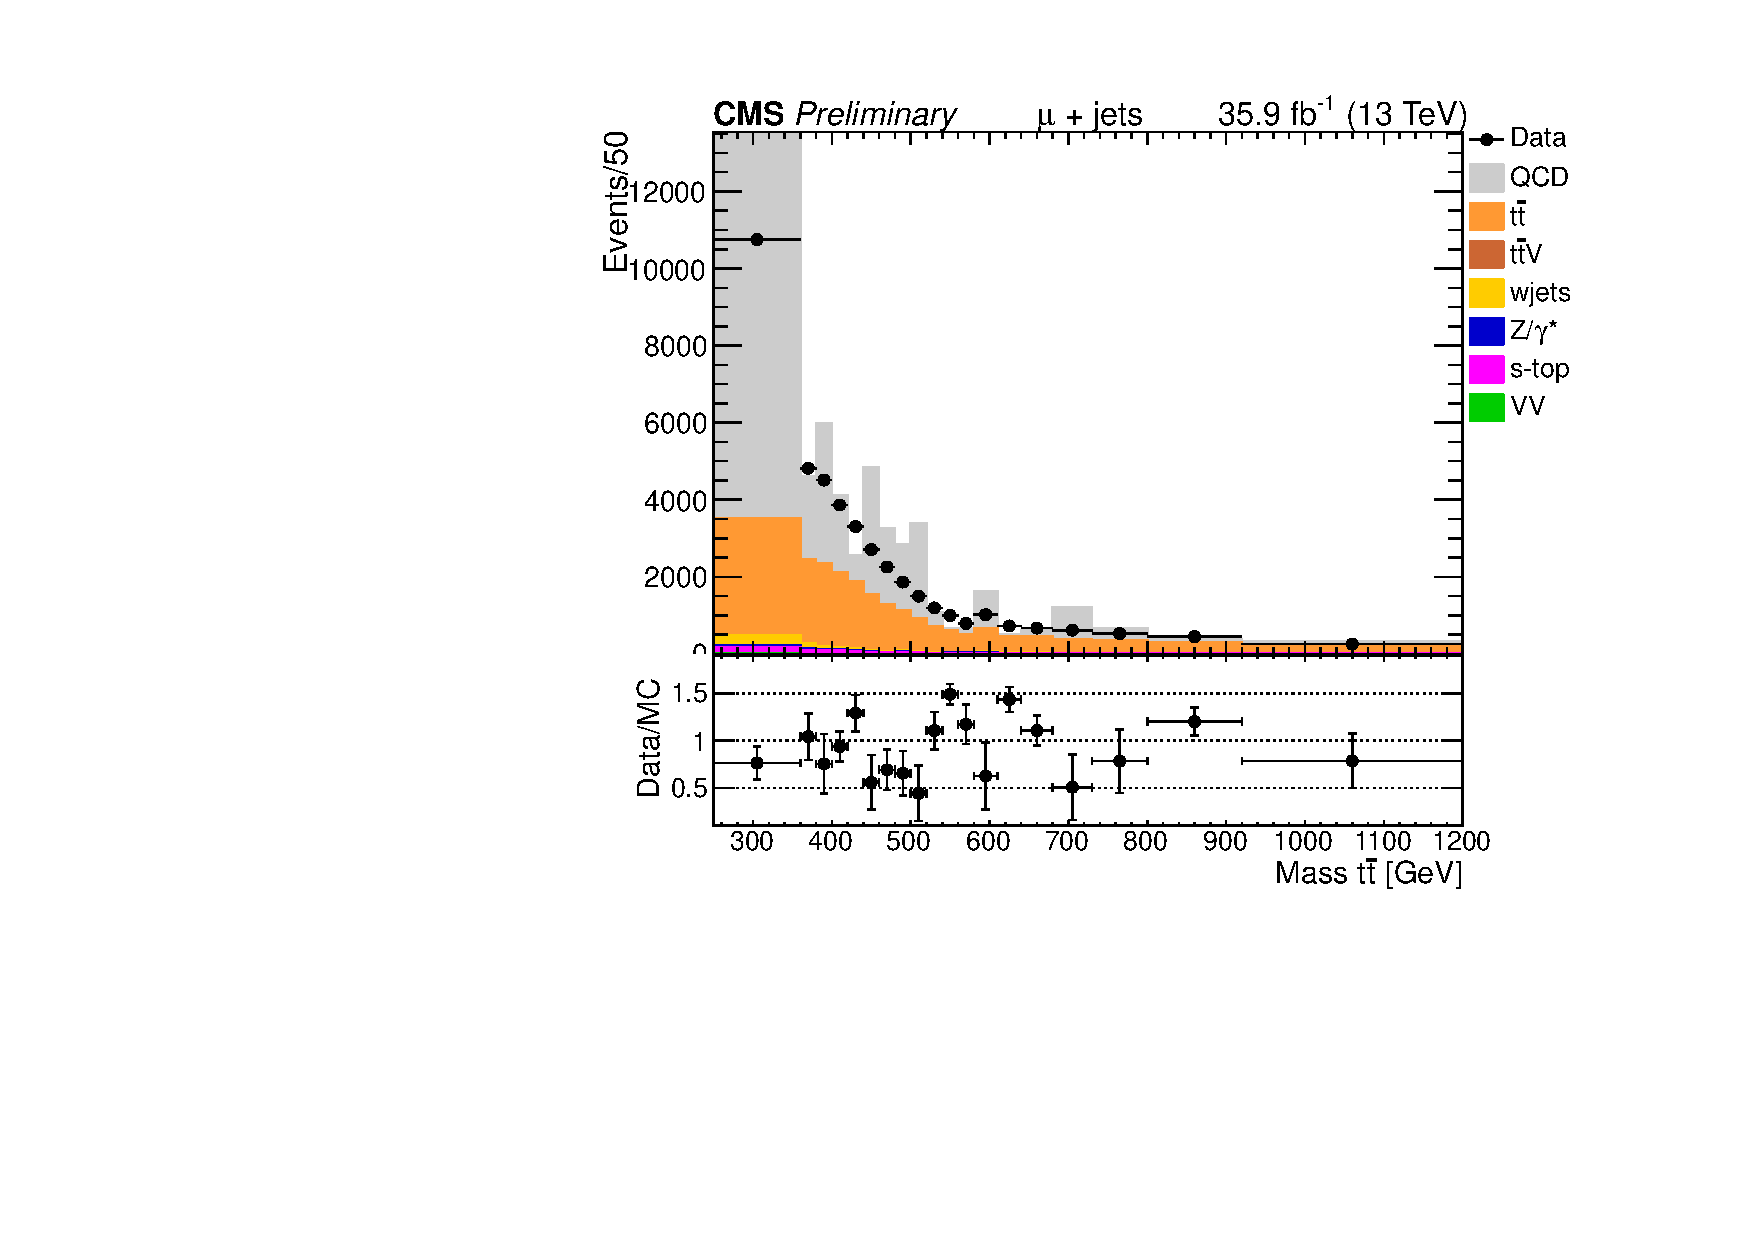
\includegraphics[scale=0.30]{fig/chapt7/qcd/qcd_mu_ch/Mass_H_binned15_24.pdf}
& \hspace{-1.20cm} 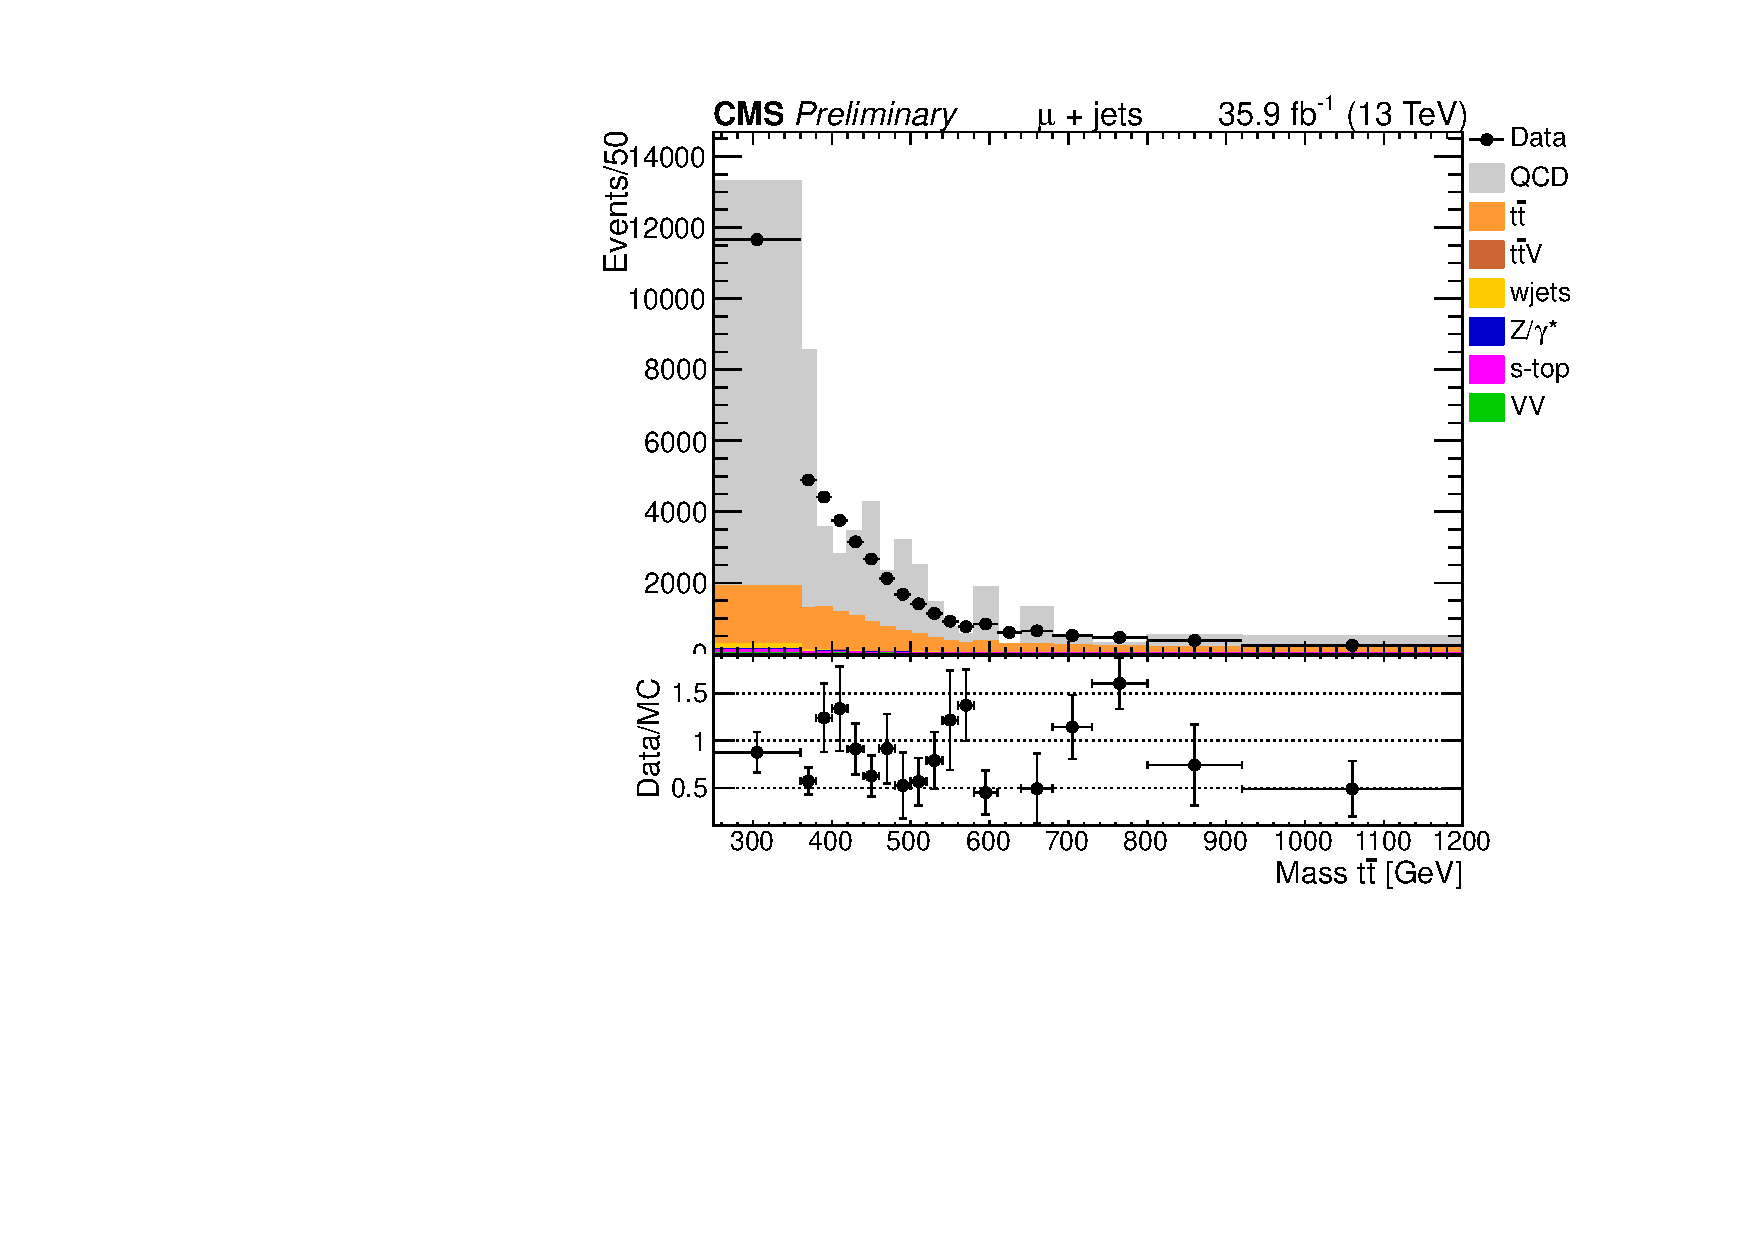
\includegraphics[scale=0.30]{fig/chapt7/qcd/qcd_mu_ch/Mass_H_binned24_43.pdf}
& \hspace{-1.20cm} 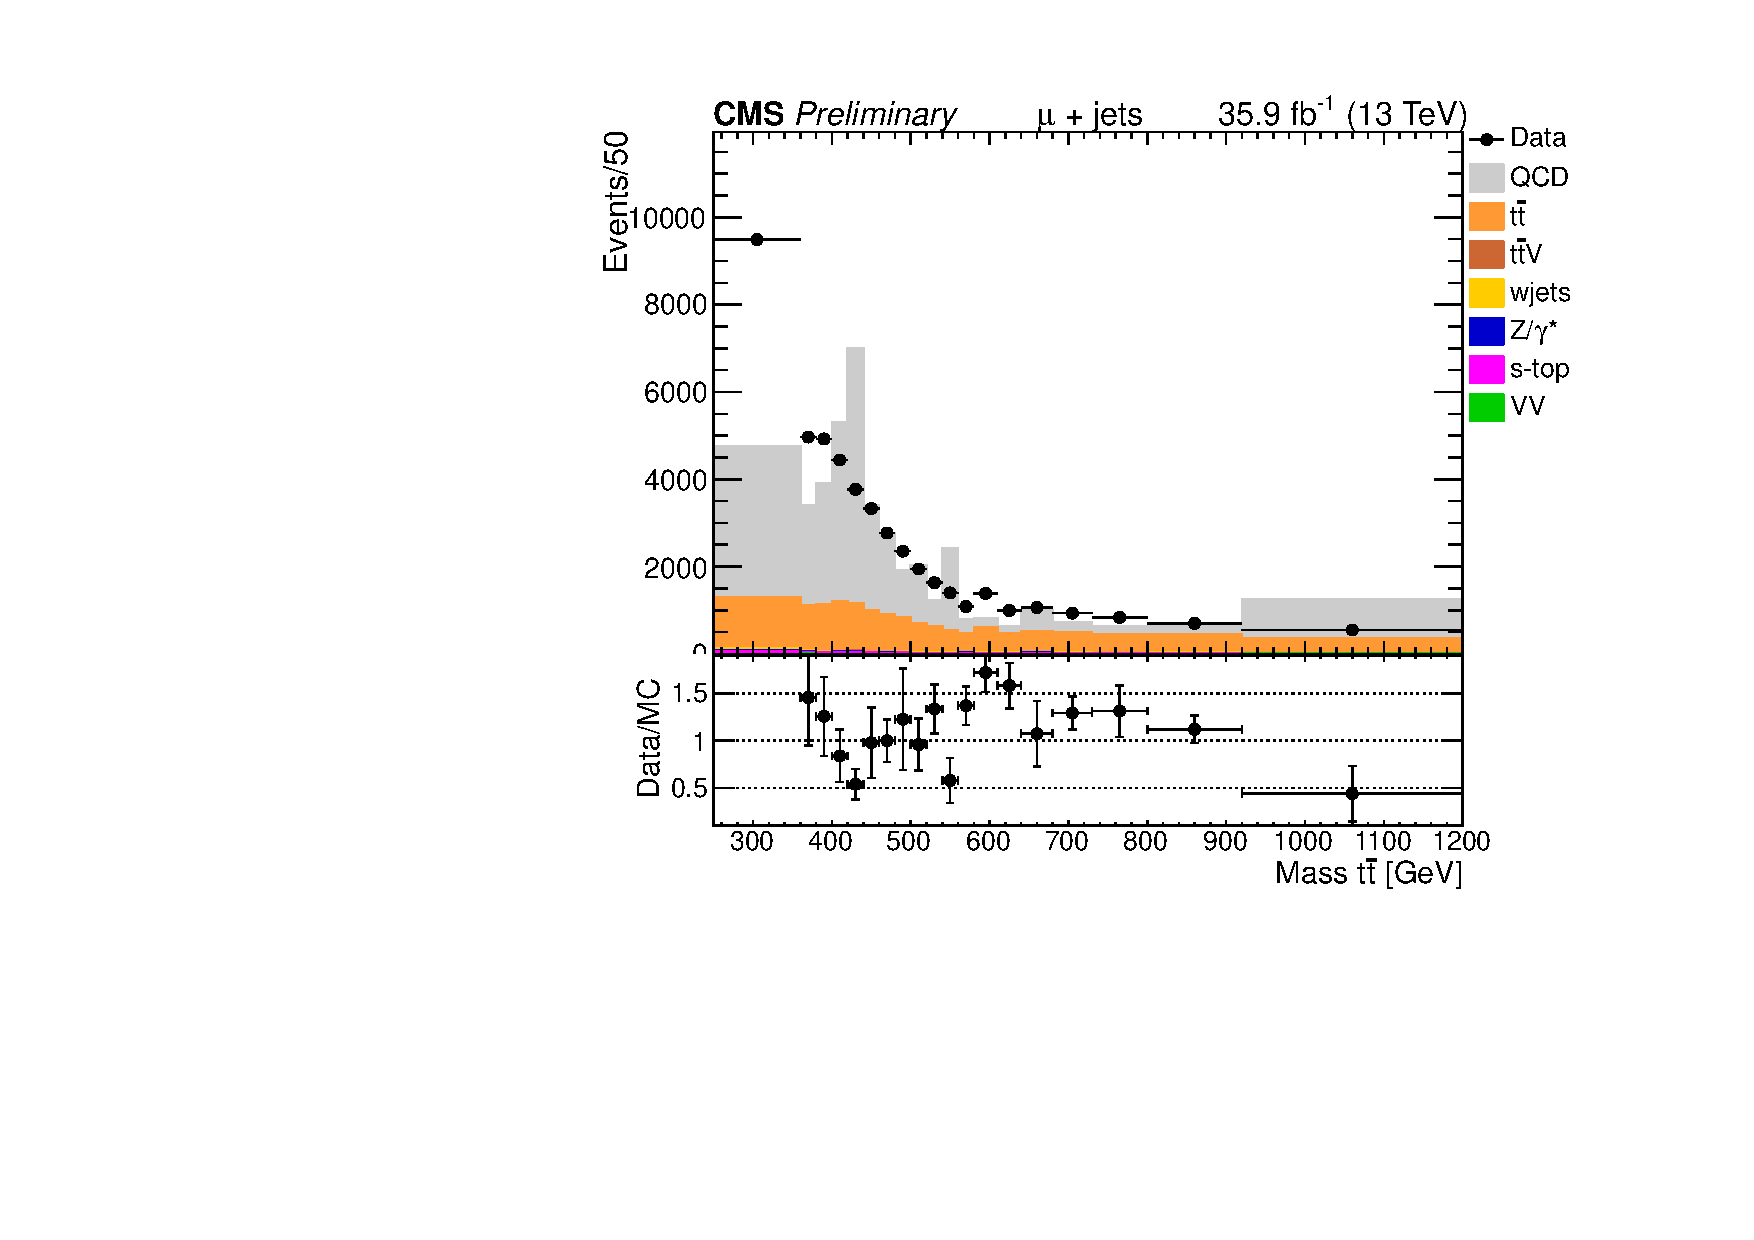
\includegraphics[scale=0.30]{fig/chapt7/qcd/qcd_mu_ch/Mass_H_binned43_Inf.pdf}\\
   ($\mathbf{a}$)\qquad\qquad&($\mathbf{b}$)\qquad\qquad\qquad&($\mathbf{c}$)\qquad\qquad\qquad\\ \\
\hspace{-0.5cm}
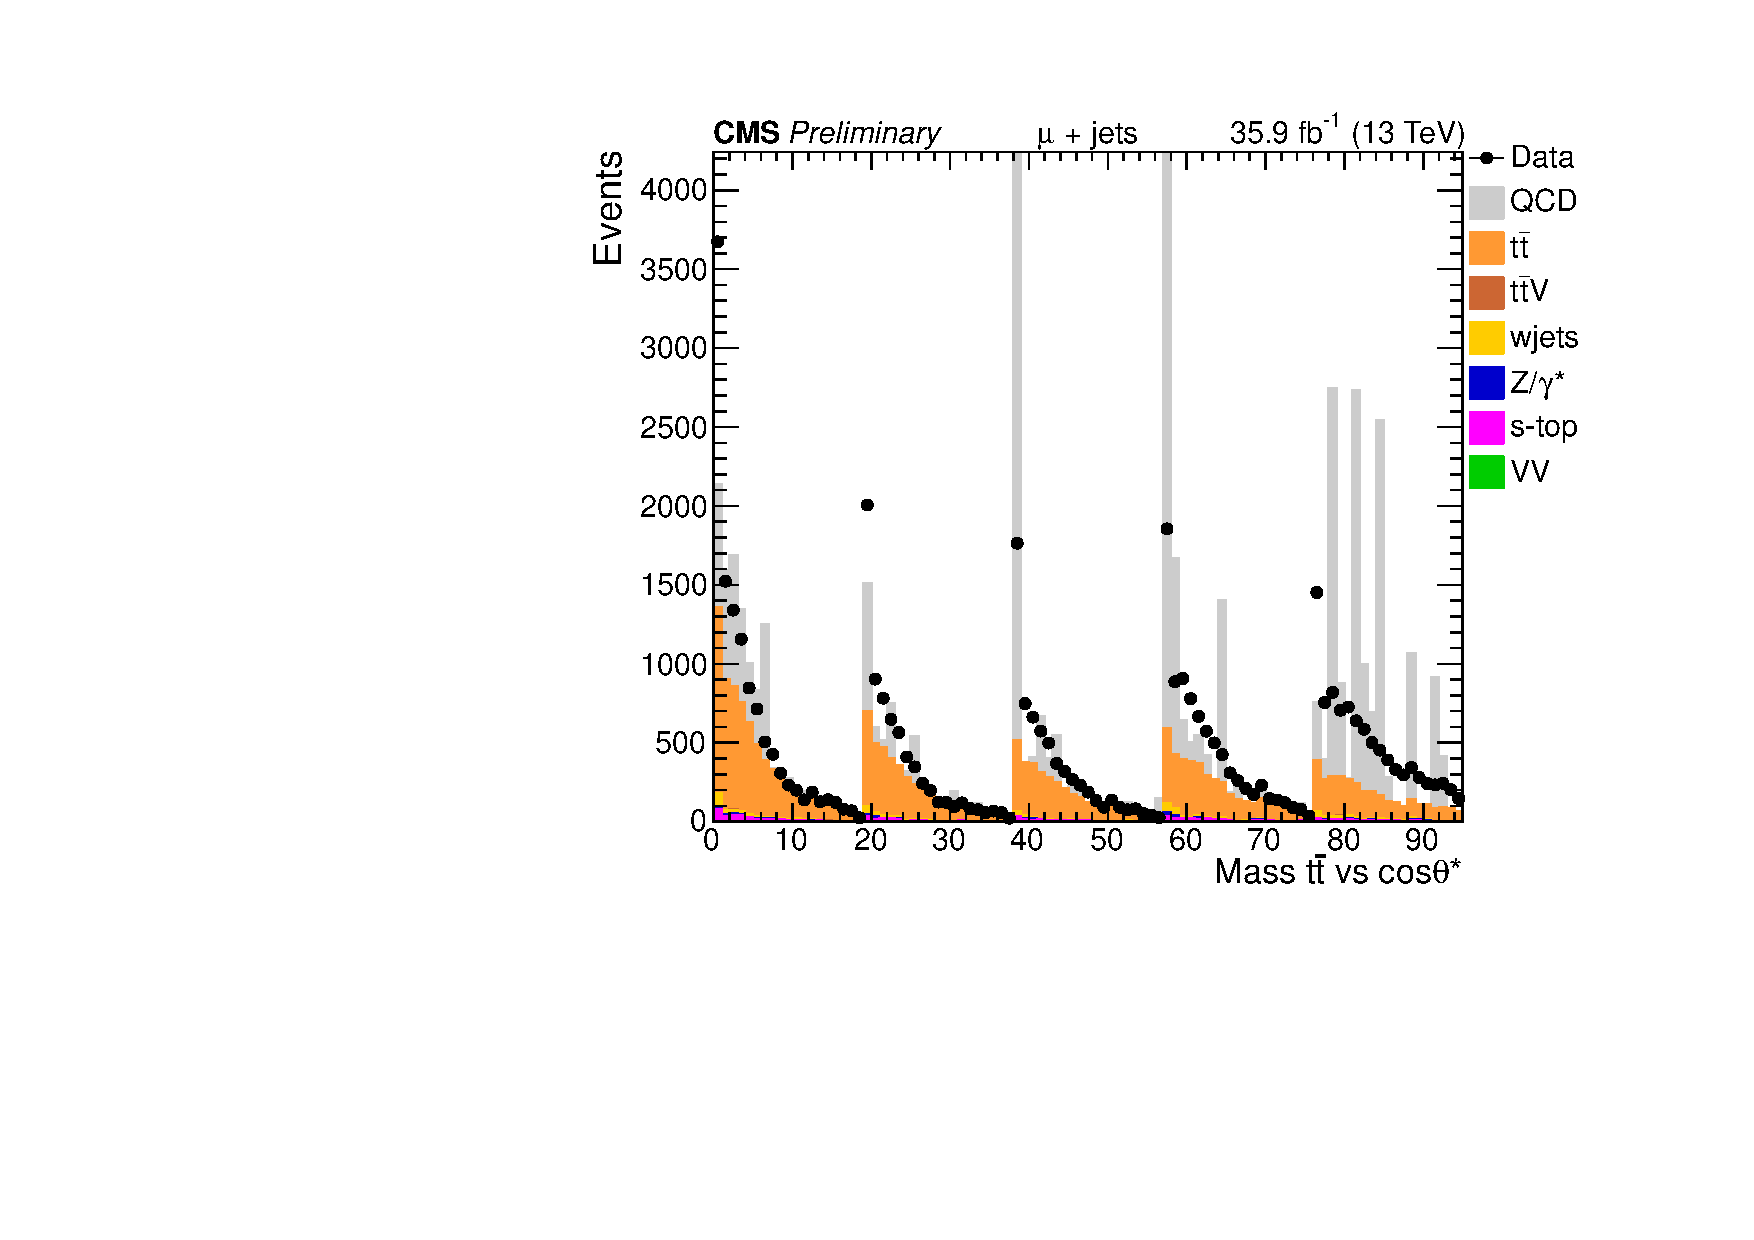
\includegraphics[scale=0.3]{fig/chapt7/qcd/qcd_mu_ch/massH_cos_theta15_24.pdf}
& \hspace{-1.2cm} 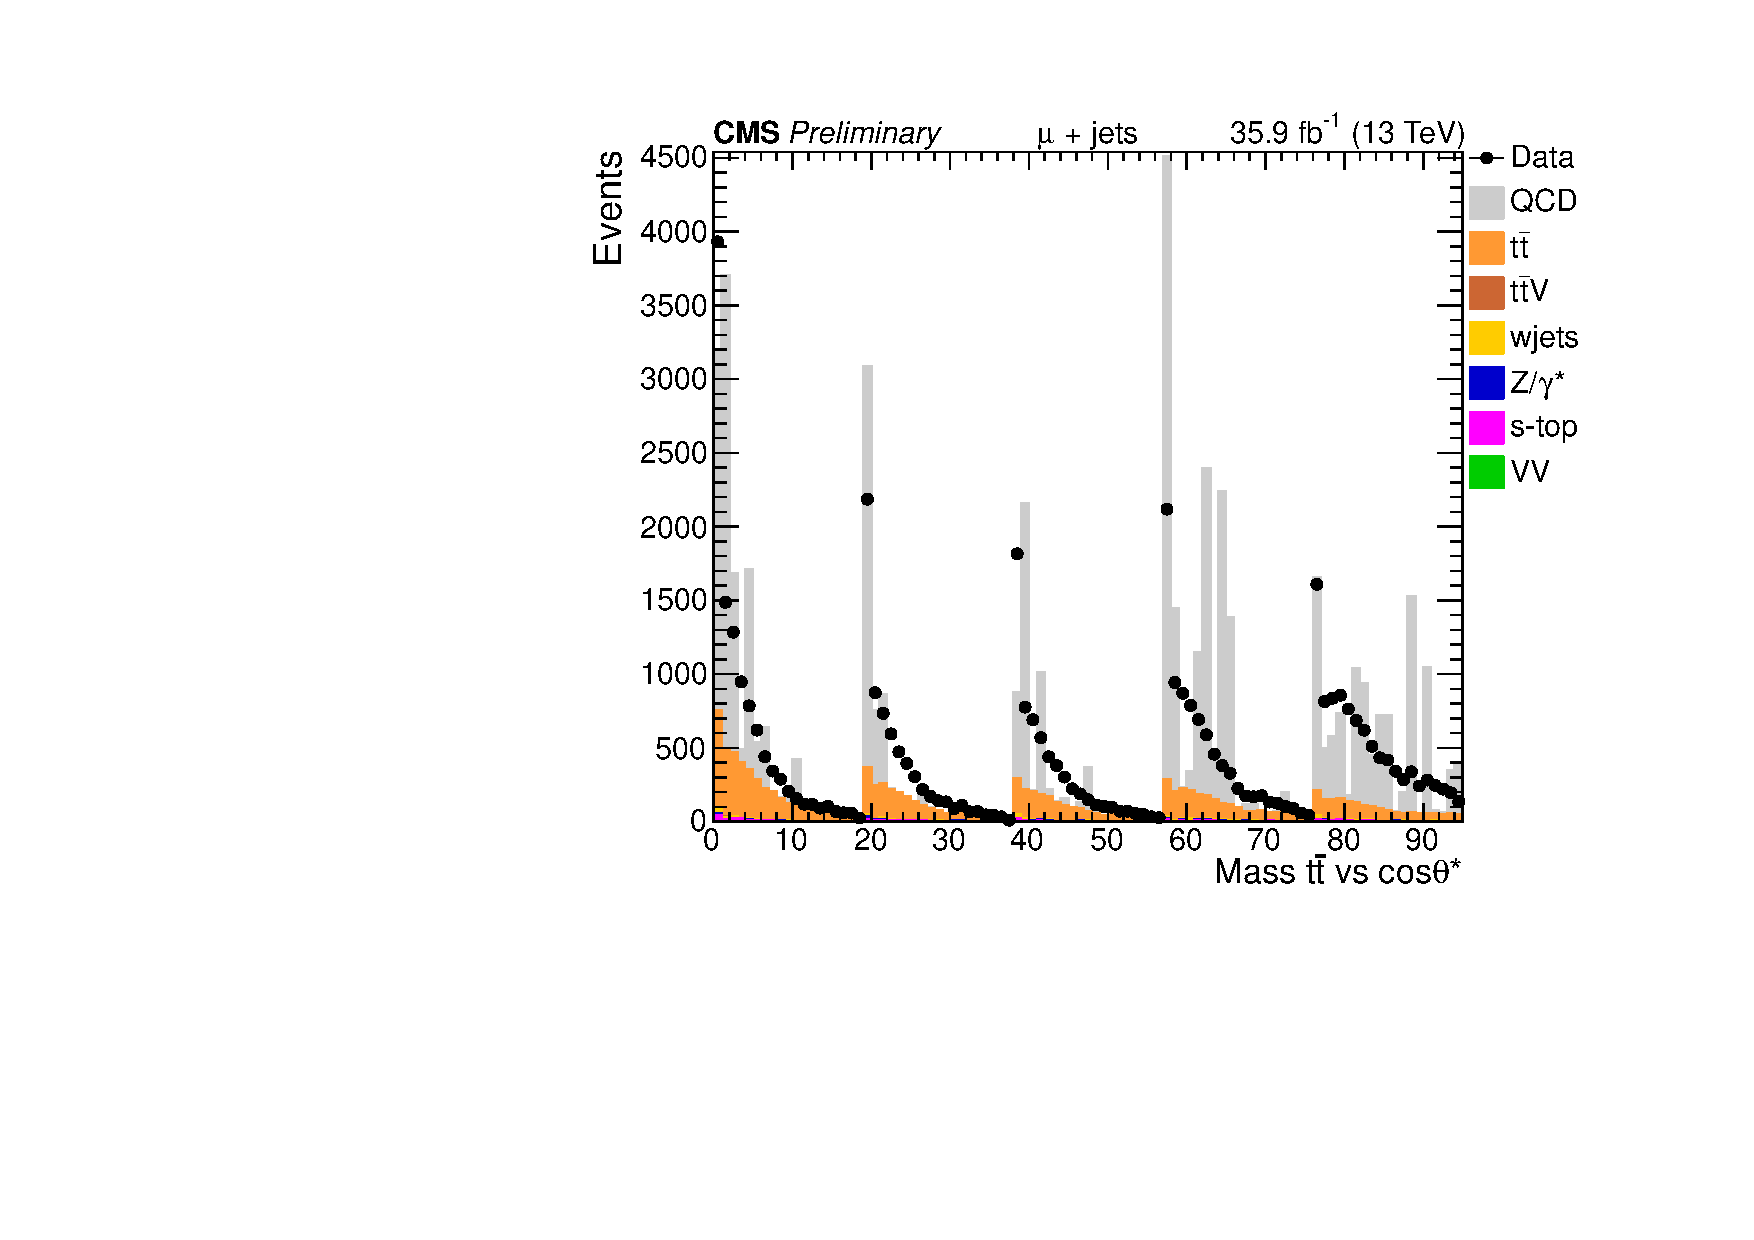
\includegraphics[scale=0.3]{fig/chapt7/qcd/qcd_mu_ch/massH_cos_theta24_43.pdf}
& \hspace{-1.2cm} 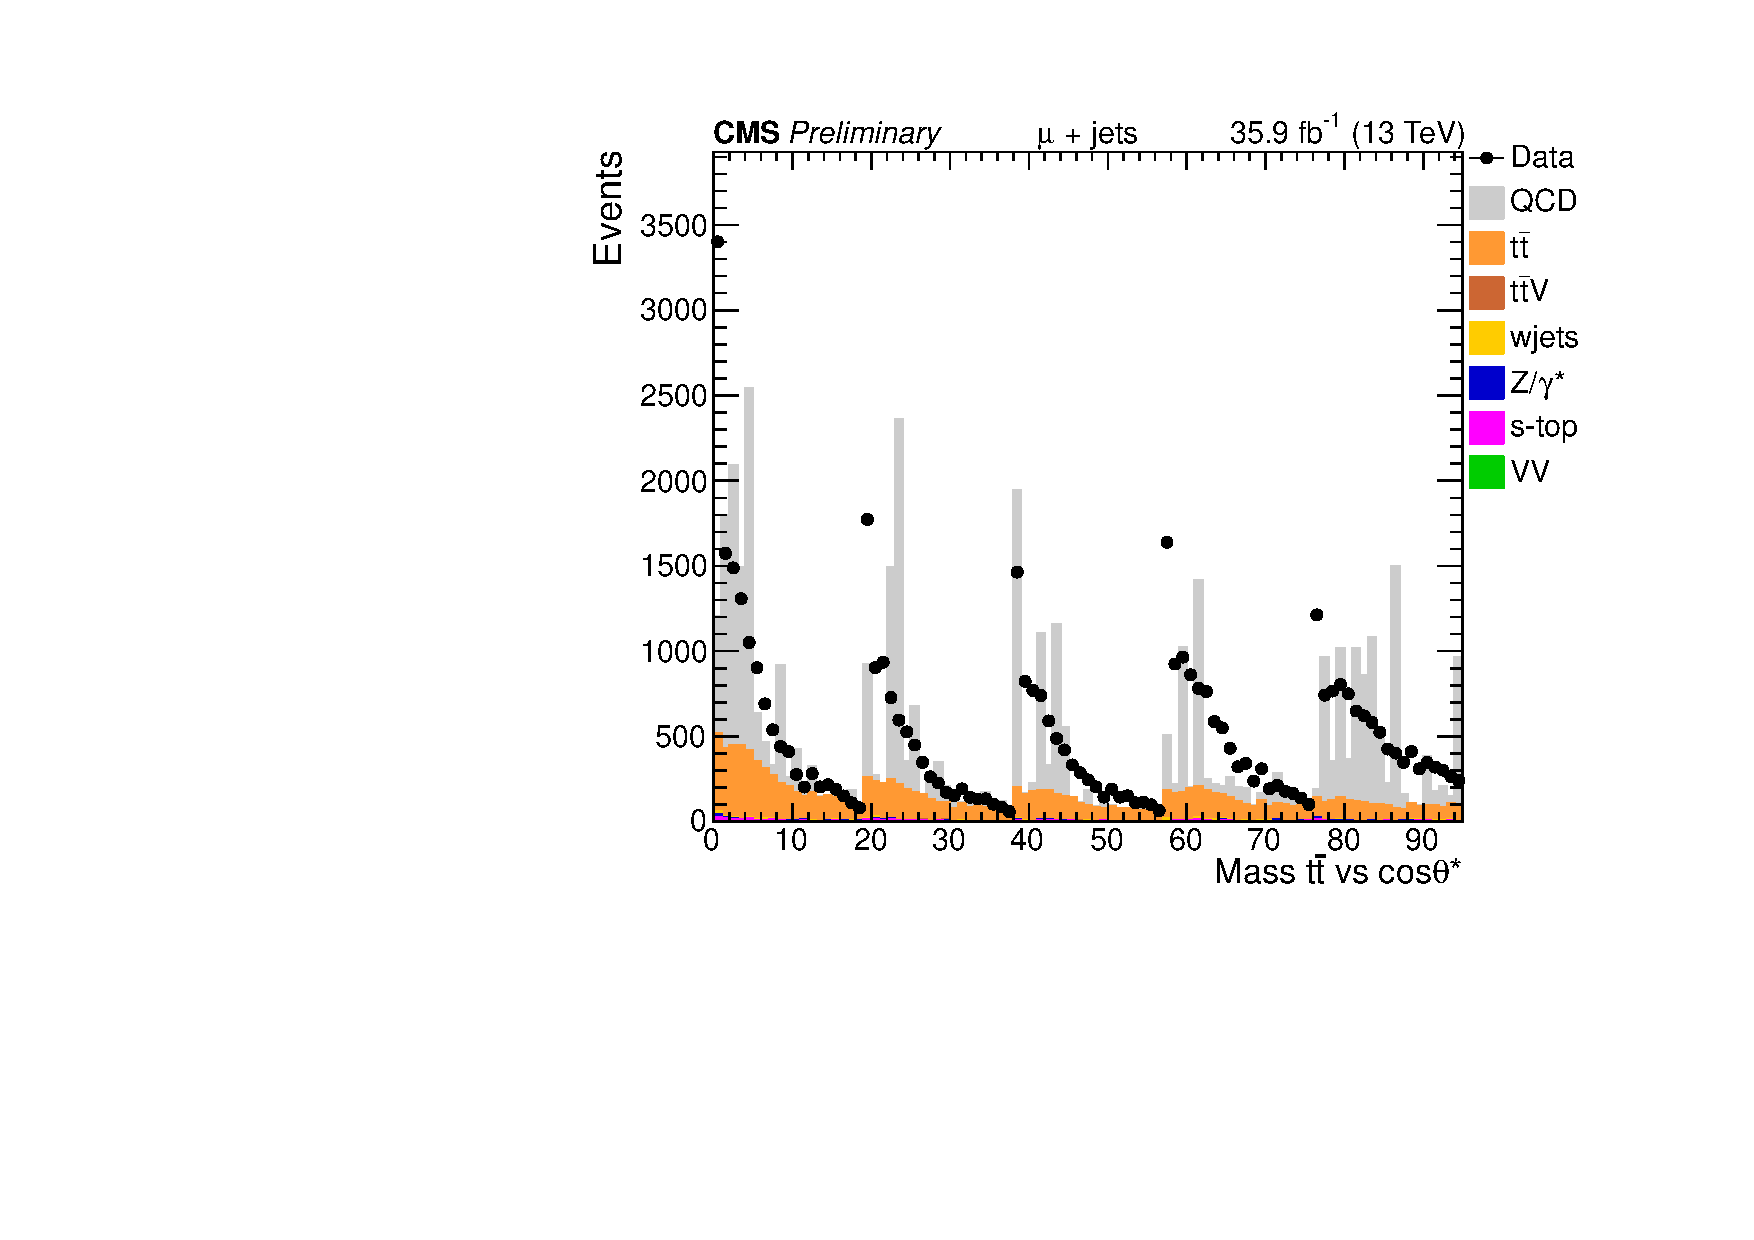
\includegraphics[scale=0.3]{fig/chapt7/qcd/qcd_mu_ch/massH_cos_theta43_Inf.pdf}\\
   ($\mathbf{d}$)\qquad\qquad&($\mathbf{e}$)\qquad\qquad\qquad&($\mathbf{f}$)\qquad\qquad\qquad\\
\hspace{-0.5cm}
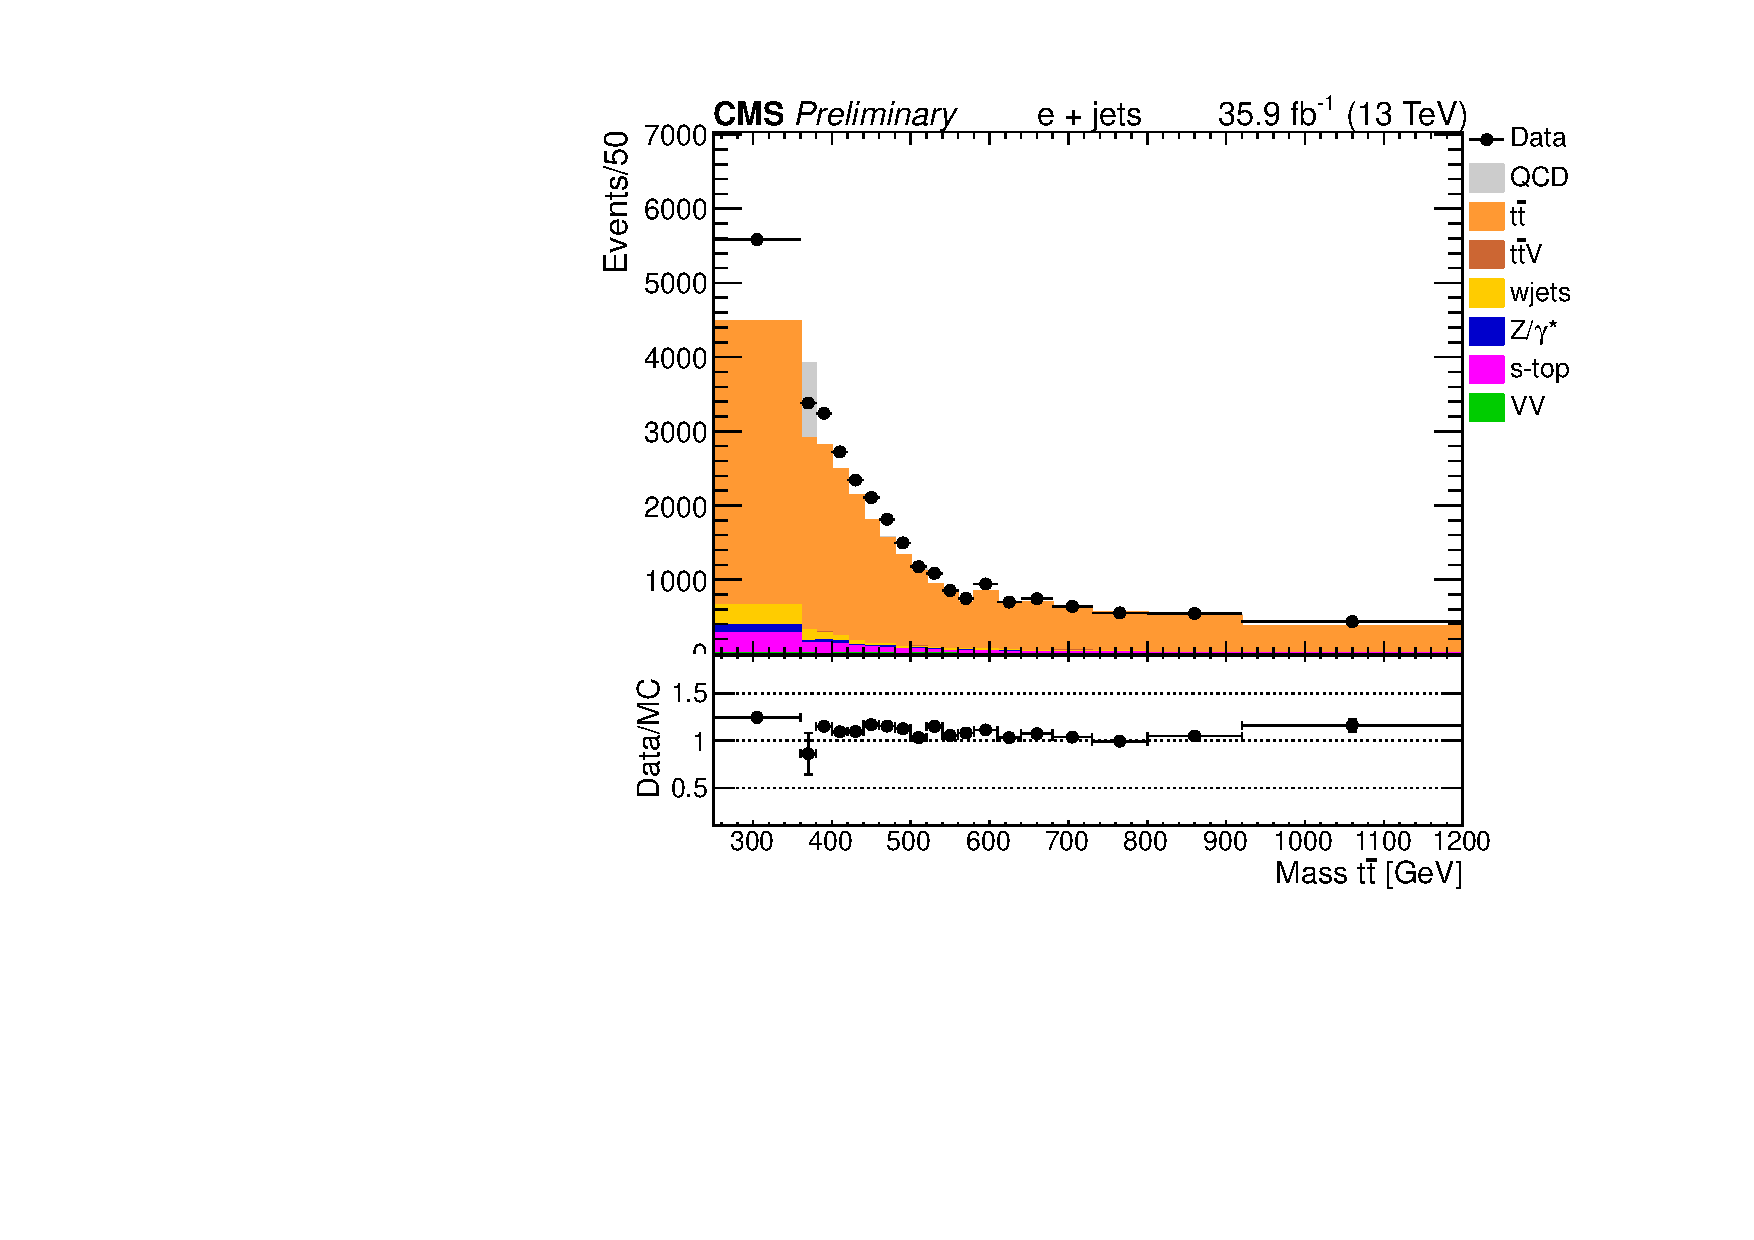
\includegraphics[scale=0.3]{fig/chapt7/qcd/qcd_e_ch/Mass_H_binned1.pdf}
& \hspace{-1.20cm} 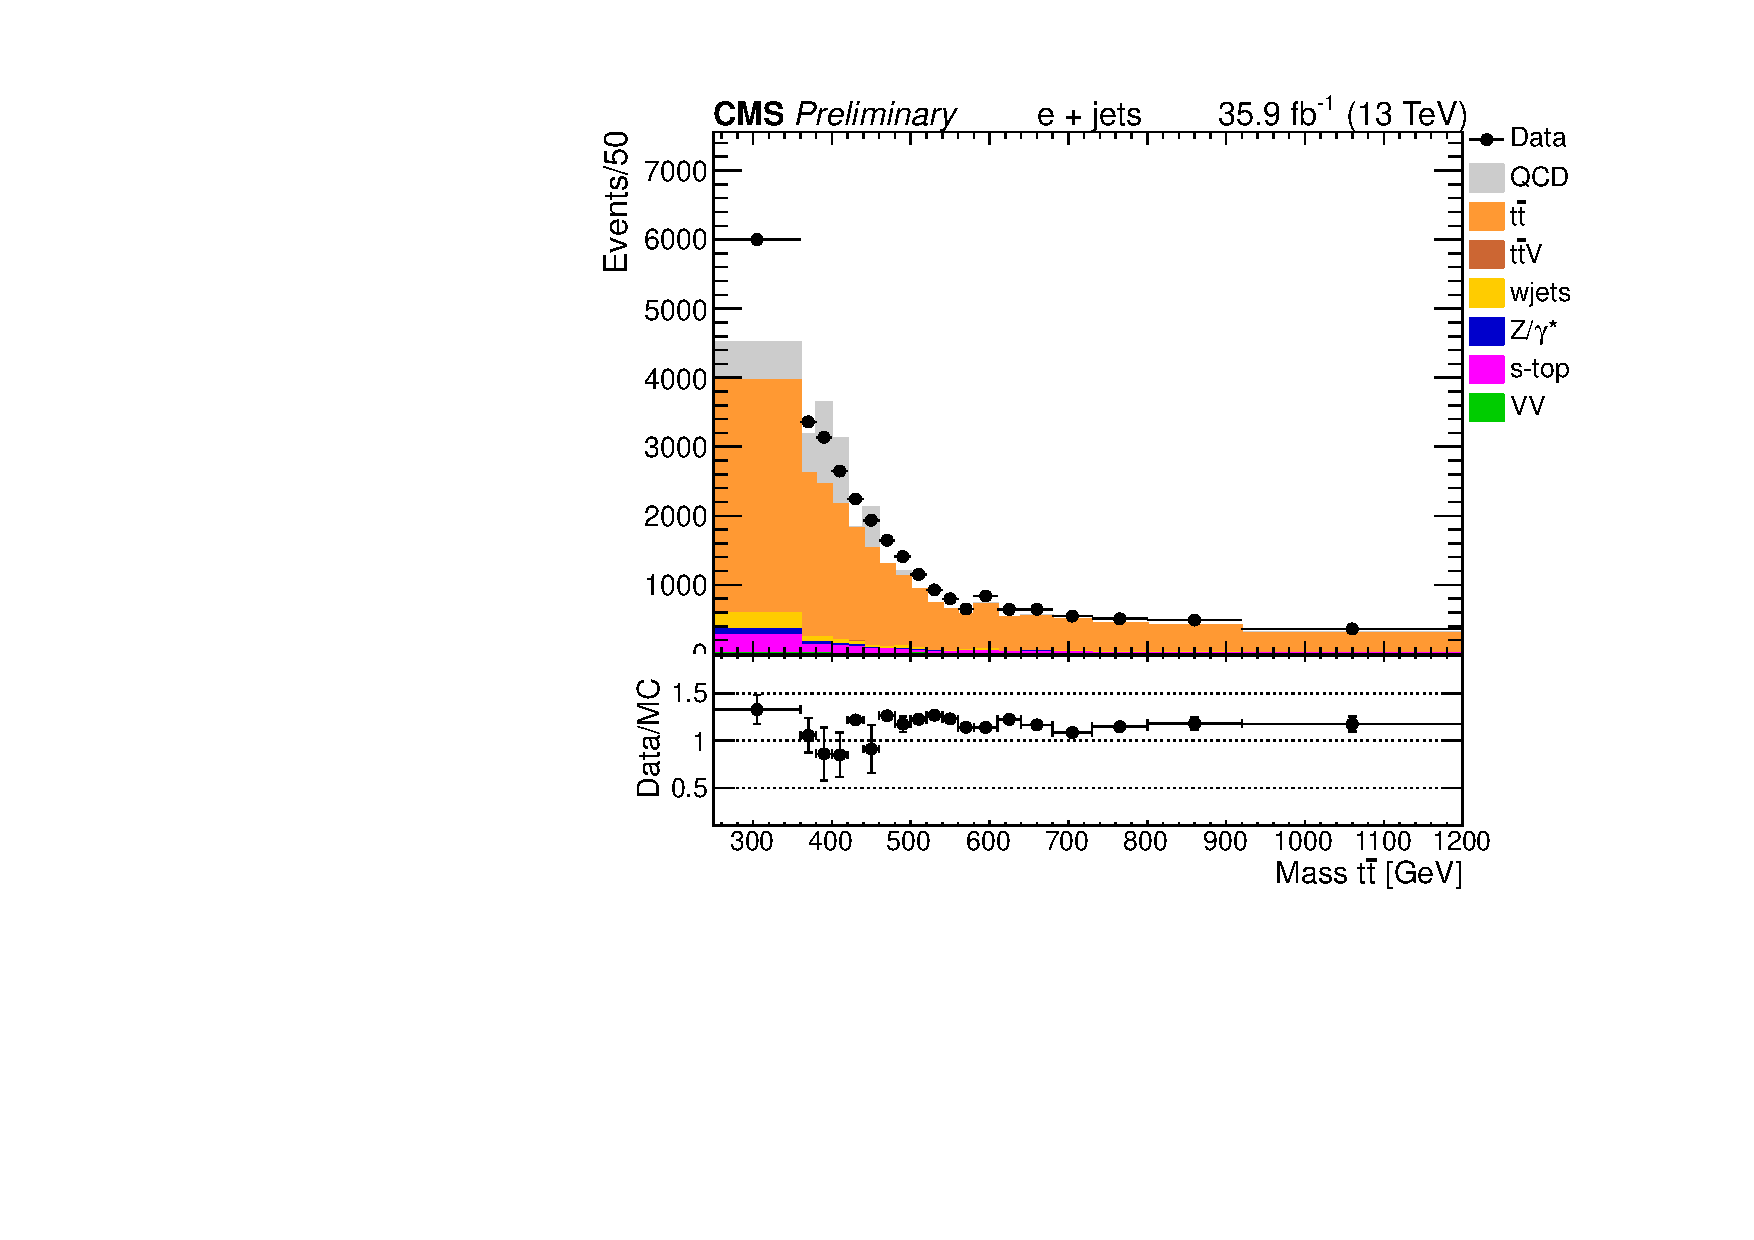
\includegraphics[scale=0.3]{fig/chapt7/qcd/qcd_e_ch/Mass_H_binned2.pdf}
& \hspace{-1.20cm} 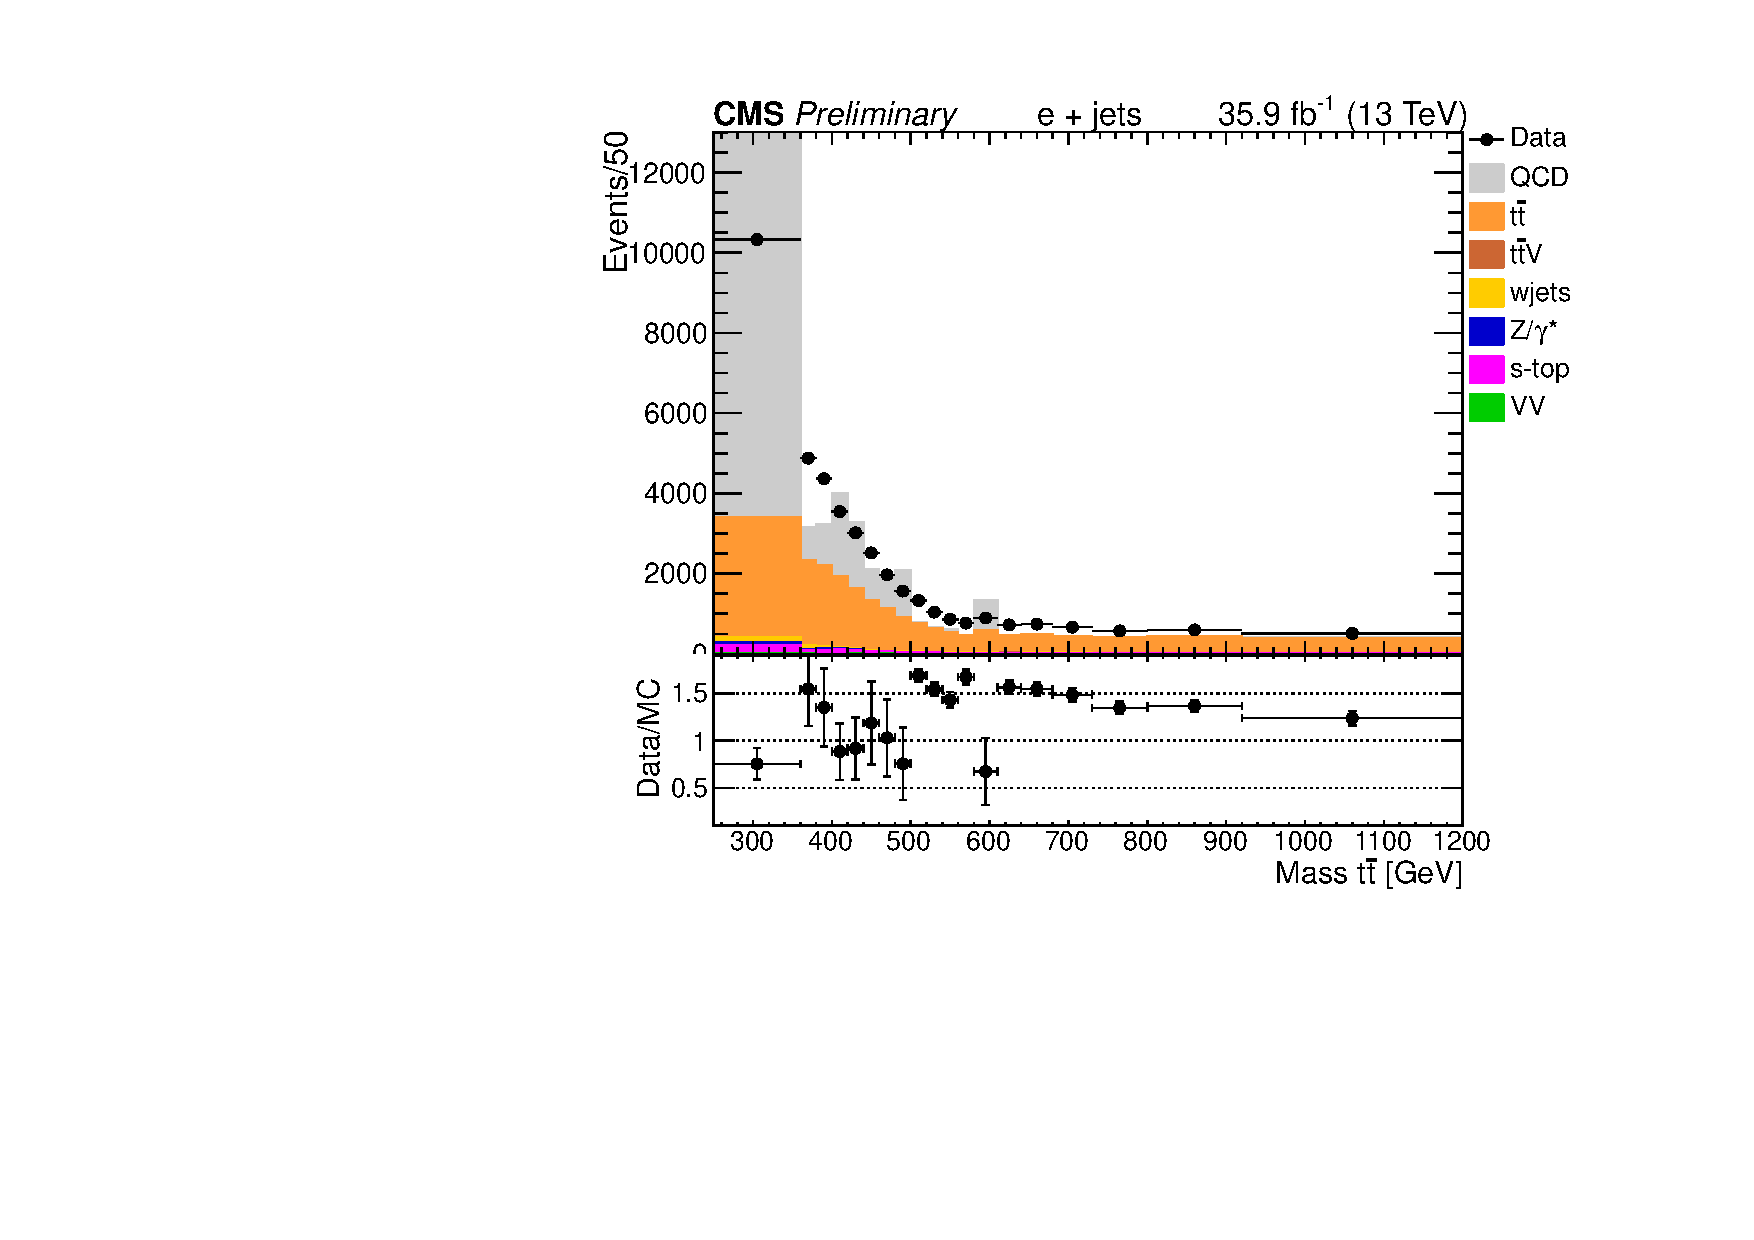
\includegraphics[scale=0.3]{fig/chapt7/qcd/qcd_e_ch/Mass_H_binned3.pdf}\\
   ($\mathbf{g}$)\qquad\qquad&($\mathbf{h}$)\qquad\qquad\qquad&($\mathbf{i}$)\qquad\qquad\qquad\\ \\
\hspace{-0.5cm}
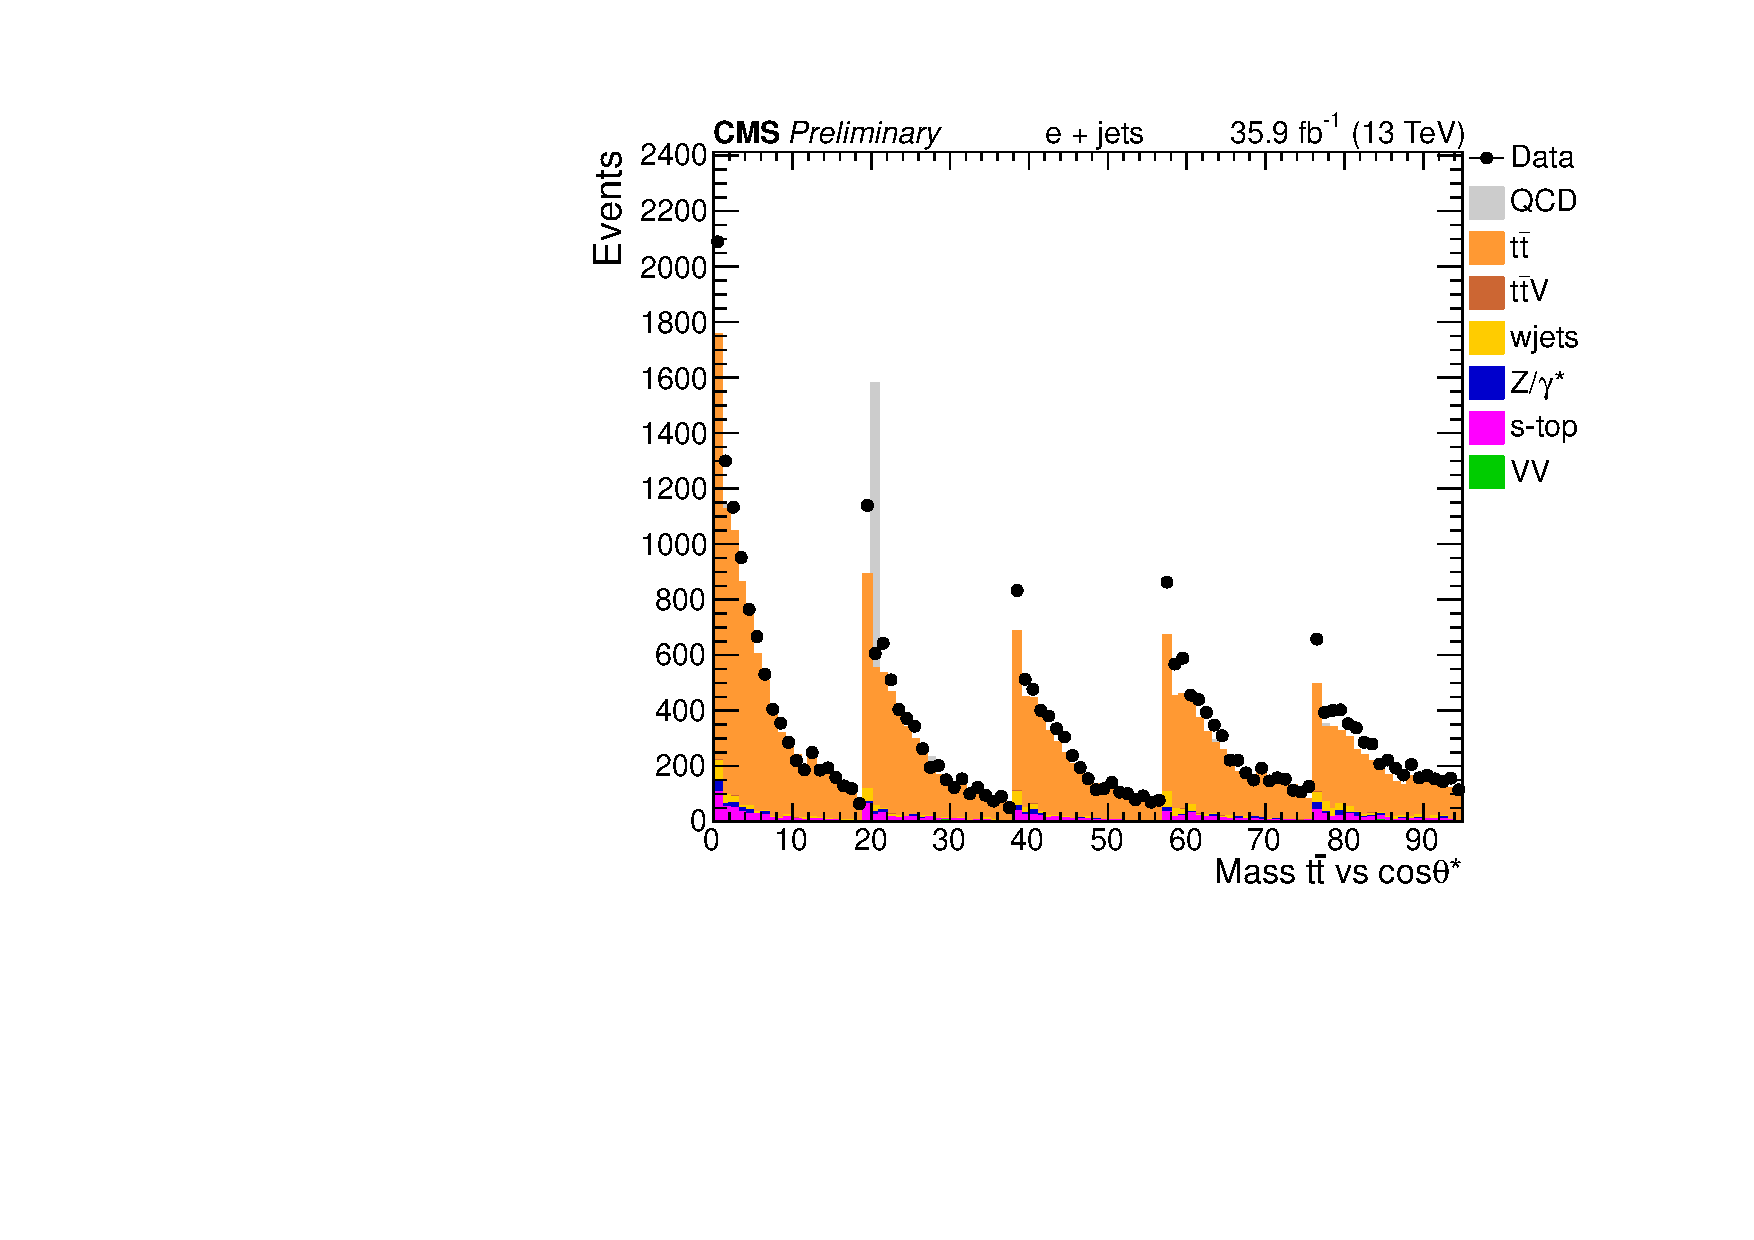
\includegraphics[scale=0.3]{fig/chapt7/qcd/qcd_e_ch/massH_cos_theta1.pdf}
& \hspace{-1.2cm} 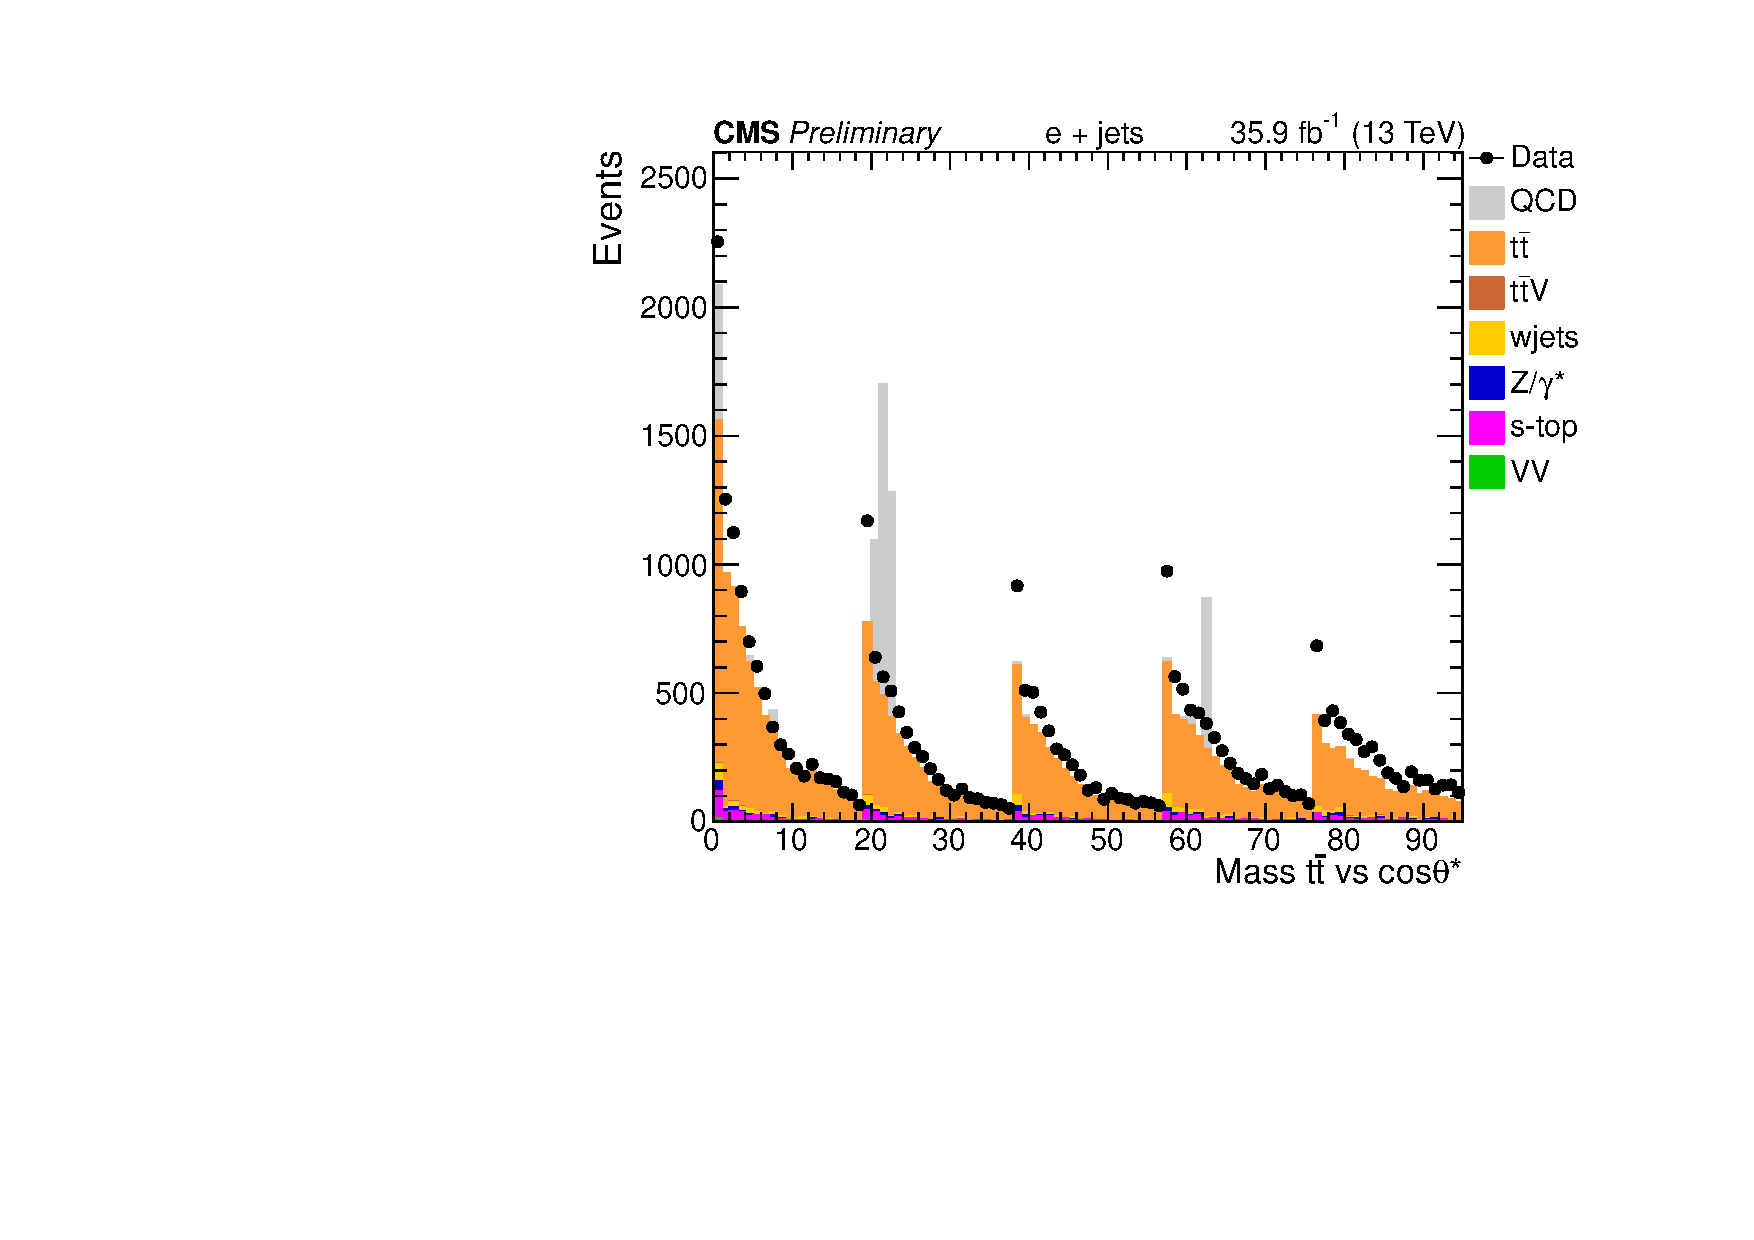
\includegraphics[scale=0.3]{fig/chapt7/qcd/qcd_e_ch/massH_cos_theta2.pdf}
& \hspace{-1.2cm} 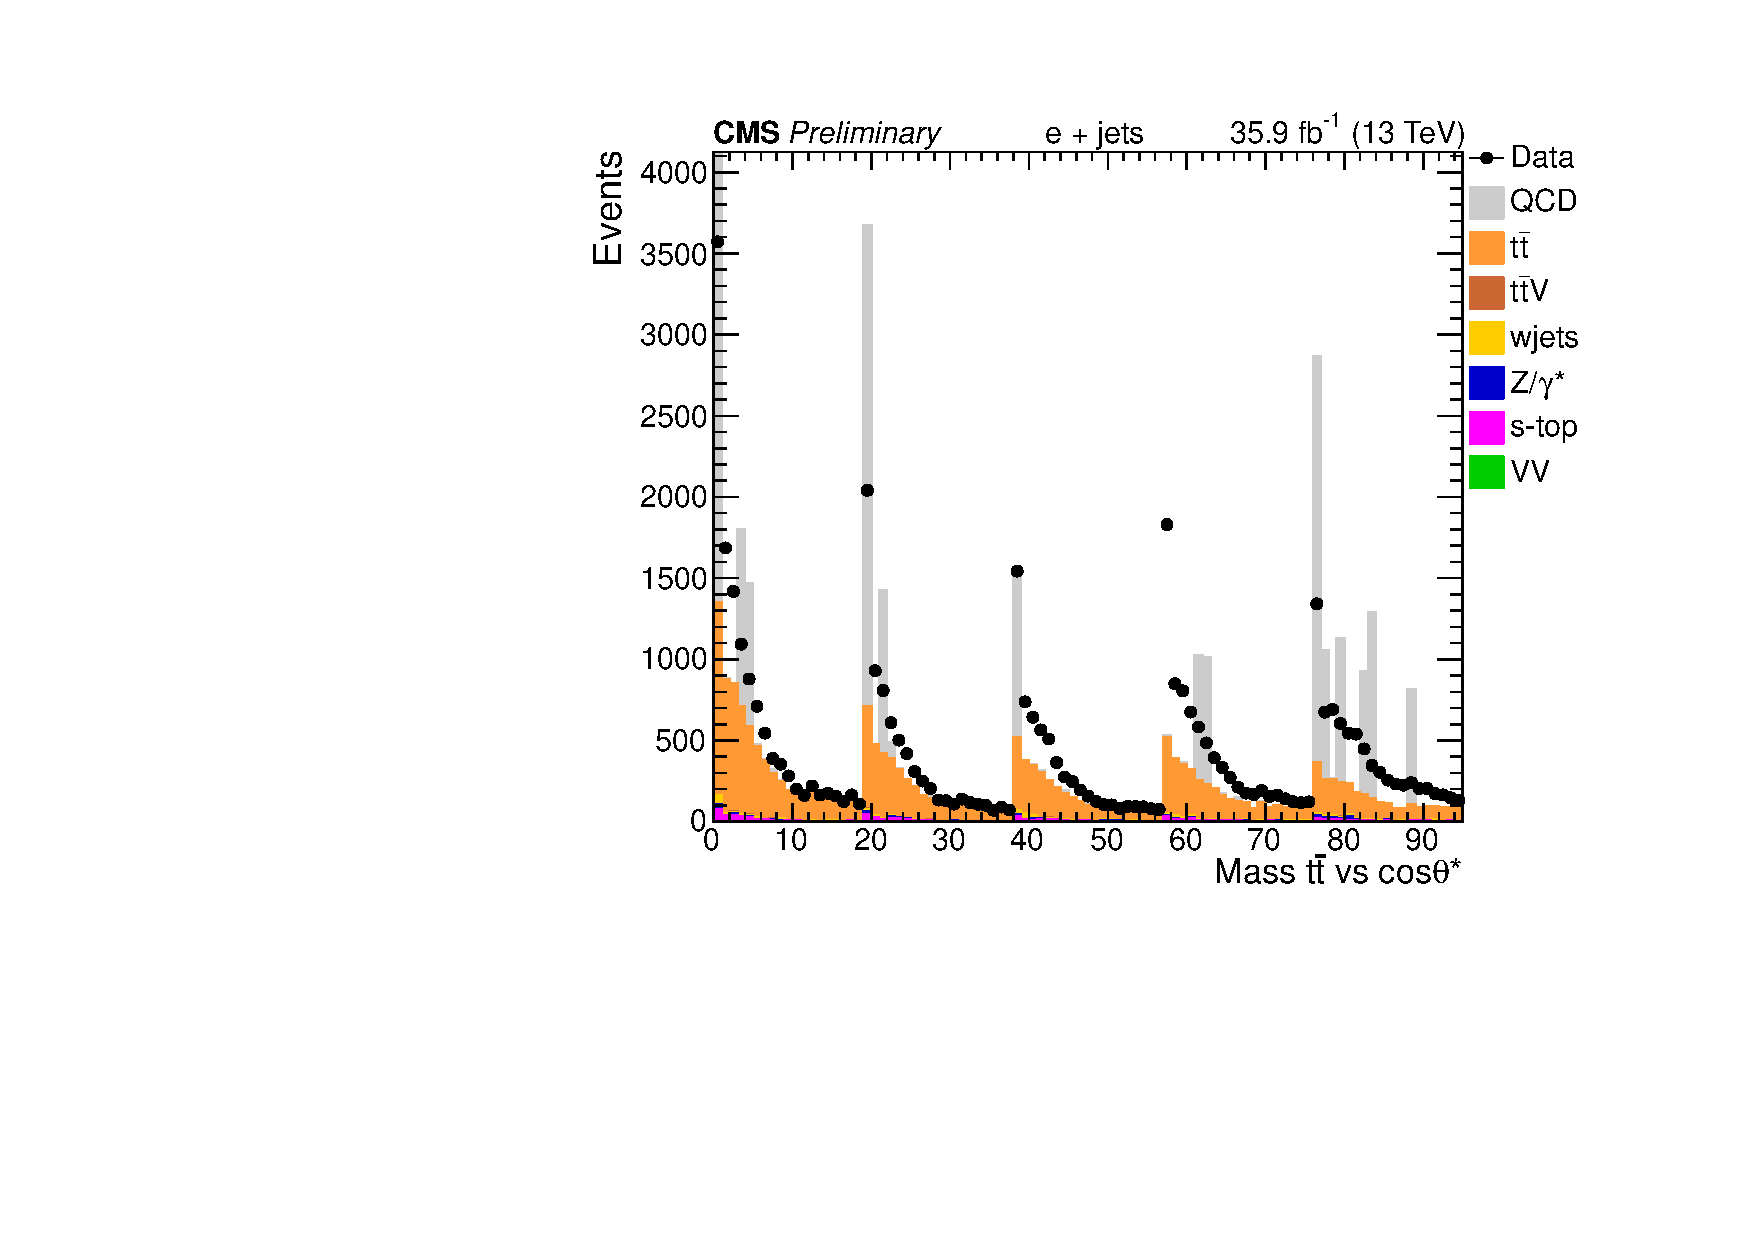
\includegraphics[scale=0.3]{fig/chapt7/qcd/qcd_e_ch/massH_cos_theta3.pdf}\\
   ($\mathbf{j}$)\qquad\qquad&($\mathbf{k}$)\qquad\qquad\qquad&($\mathbf{l}$)\qquad\qquad\qquad\\
\end{tabular}
\caption{Shape comparison of $t\overline{t}$ mass (first row) and $t\overline{t}$ mass versus cos$\theta$* (second row) for Data and MC in $\mu$-channel using three isolation regions: $0.15 \leq I_{rel}^{\mu}(\Delta\beta) < 0.24$ (first column), $0.24 \leq I_{rel}^{\mu}(\Delta\beta) < 0.43$ (second column) and $0.43 \leq I_{rel}^{\mu}(\Delta\beta)$ (last column).\\
For electron channel, third row represents $t\overline{t}$ mass and fourth row $t\overline{t}$ mass versus cos$\theta$* where the isolation regions are: $0.0588 \leq I(\rho) < 0.083$ for barrel and $0.0571 \leq I(\rho) < 0.083$ for endcap in the first column. $0.083 \leq I(\rho) < 0.13$ both for barrel and endcap in the second column and $0.13 \leq I(\rho)$ in third column.}
\label{Fig:qcd_3region_shapes}
\end{figure}
%-----------------------------
\begin{figure}[htp]
%\centering
\begin{tabular}{cccc}
\hspace{-0.5cm}
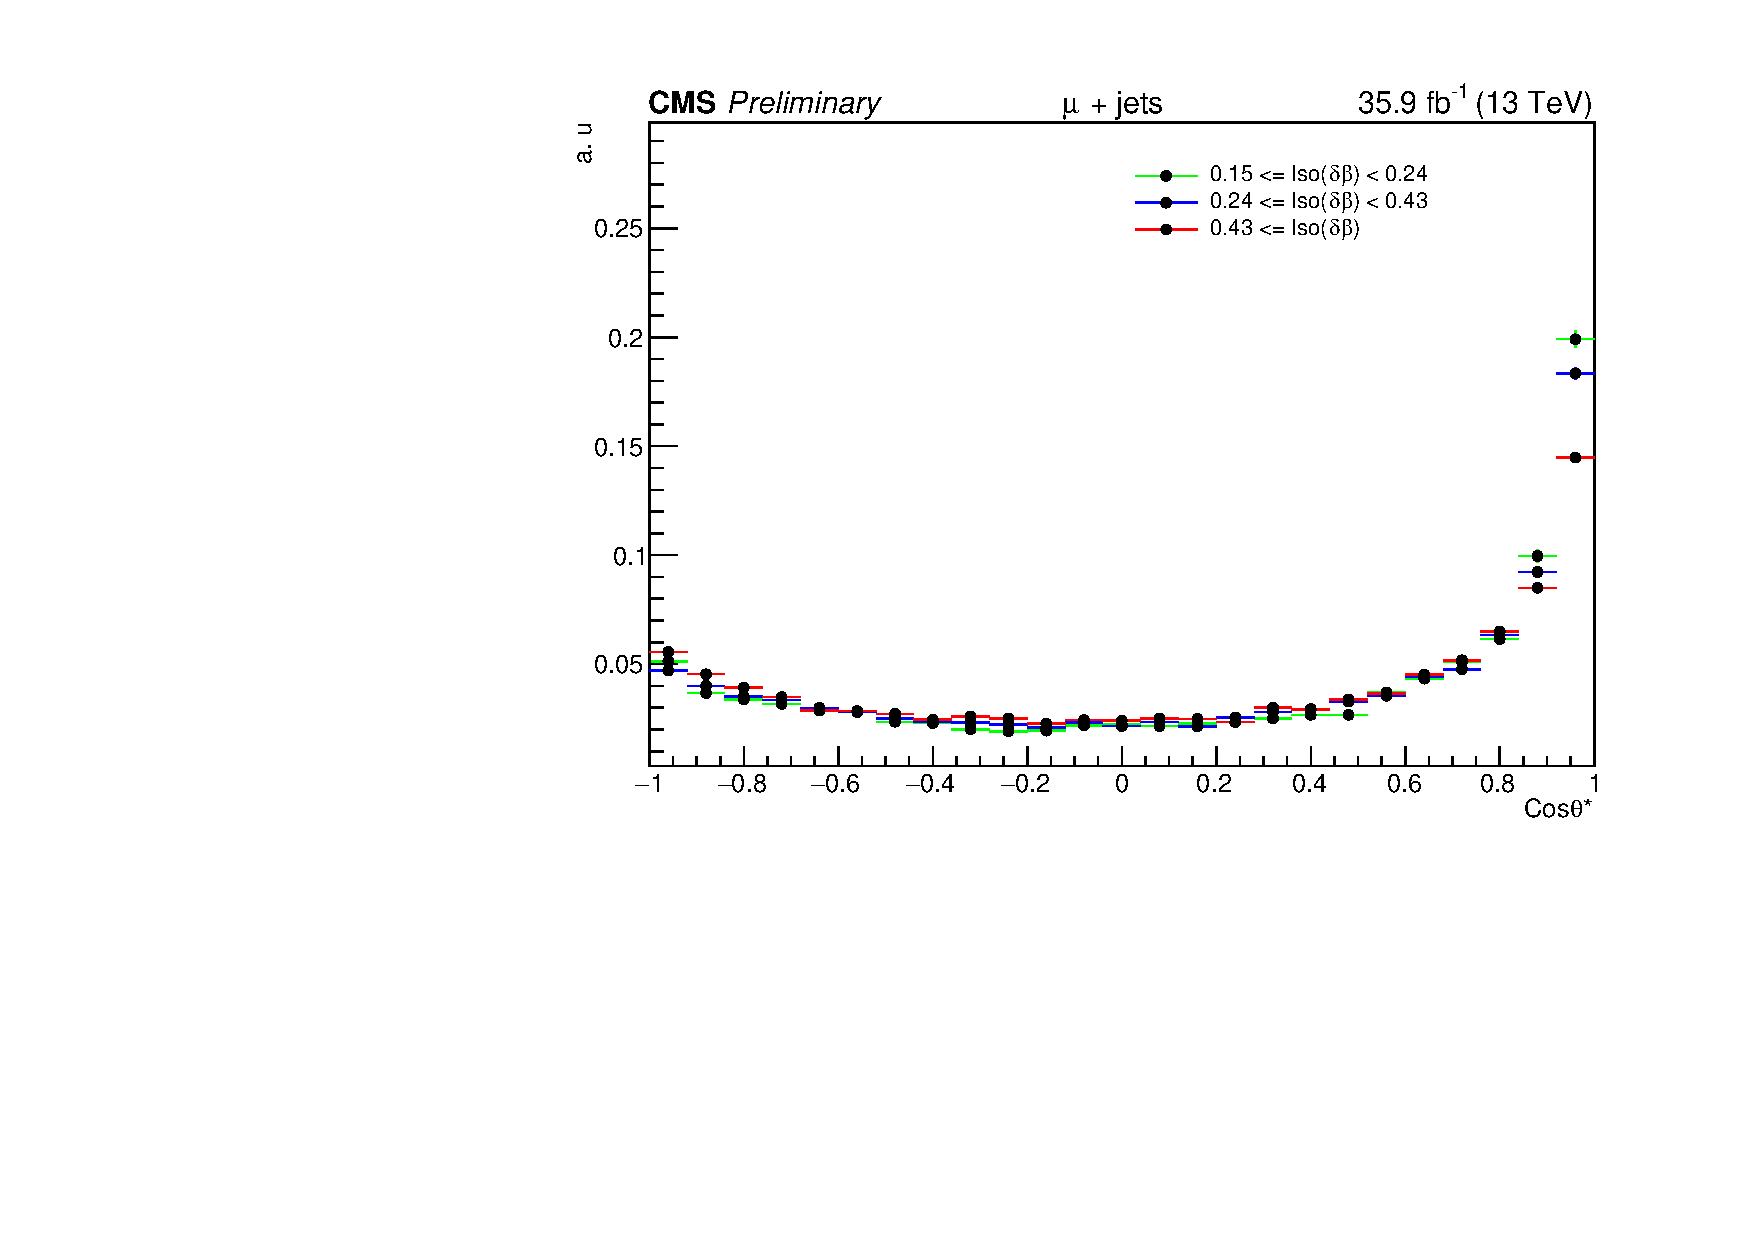
\includegraphics[scale=0.21]{fig/chapt7/qcd/qcd_mu_ch/cosine_3region_compare.pdf}
& \hspace{-0.95cm} 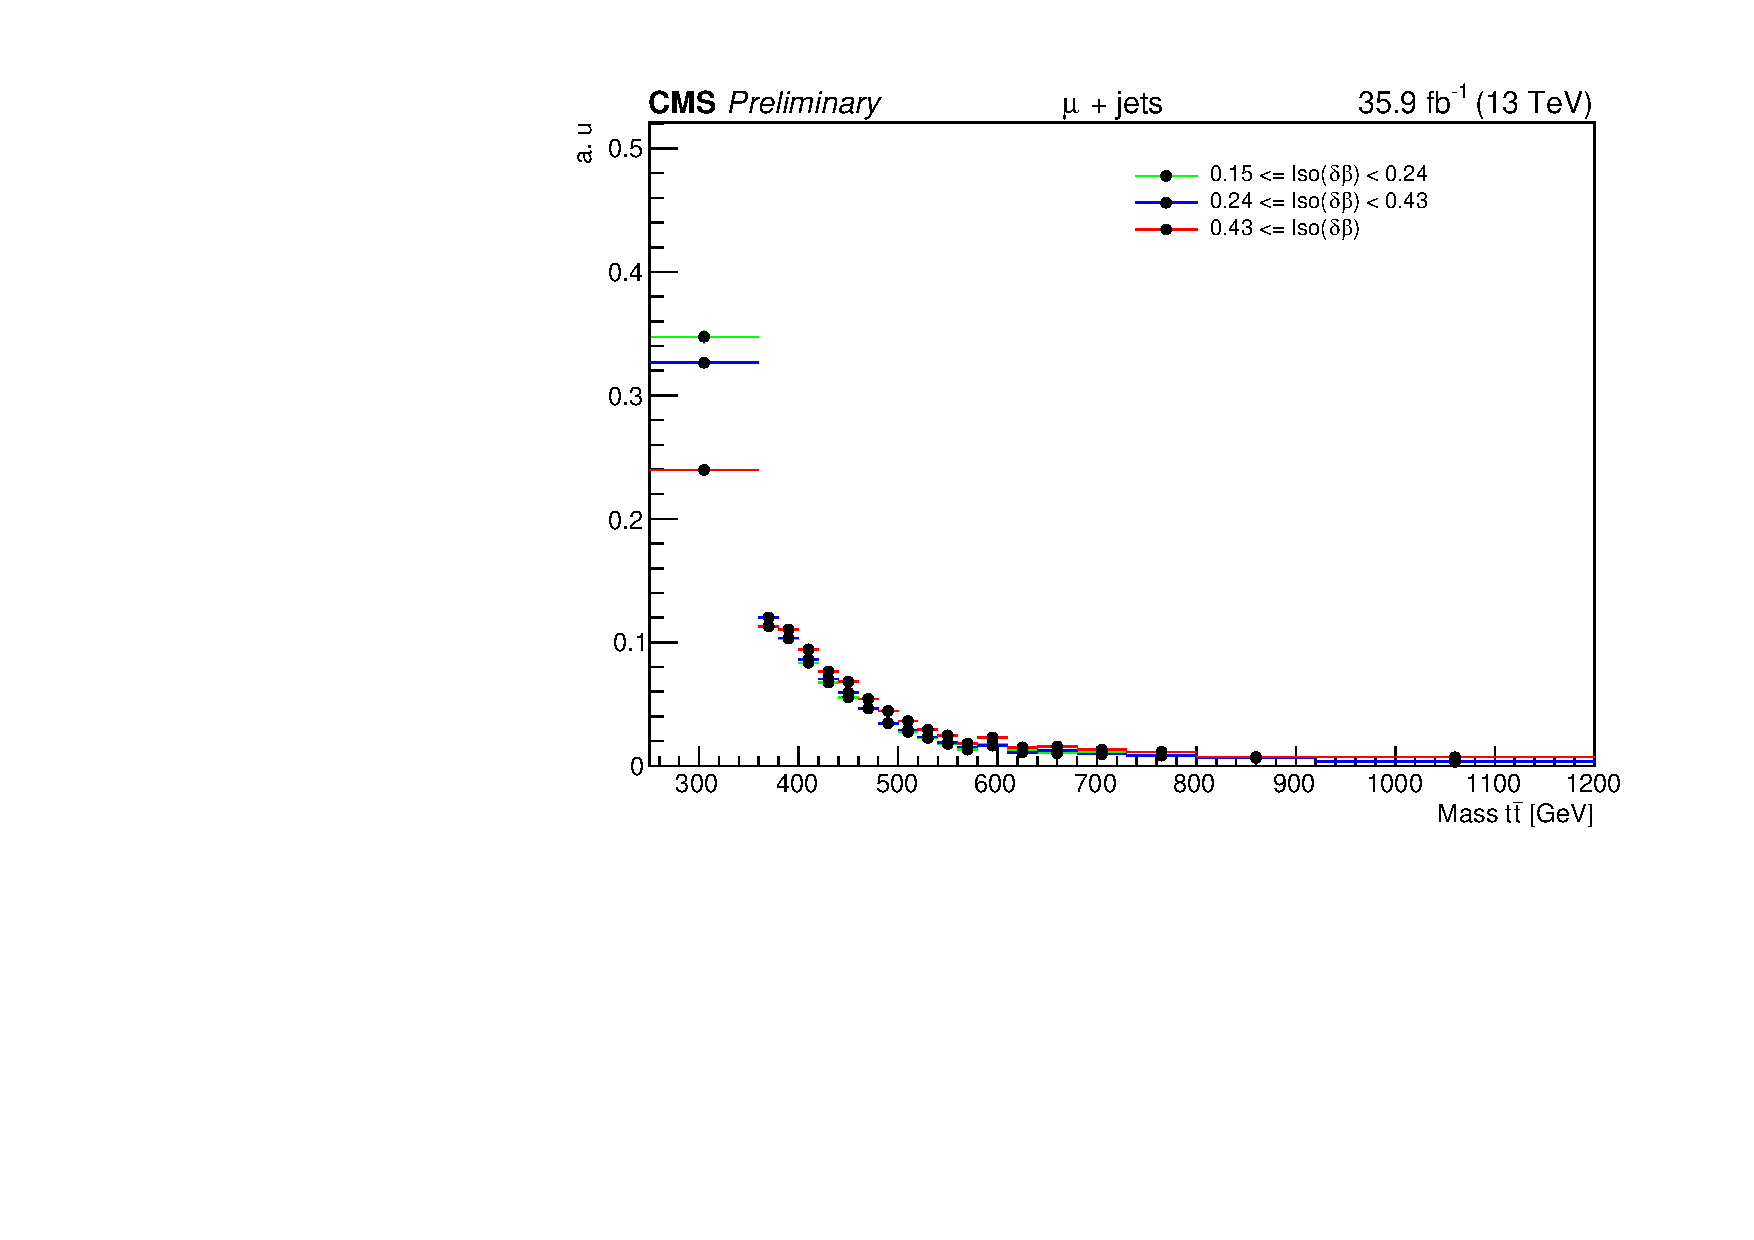
\includegraphics[scale=0.21]{fig/chapt7/qcd/qcd_mu_ch/ttbar_m_3region_compare.pdf}
& \hspace{-0.95cm} 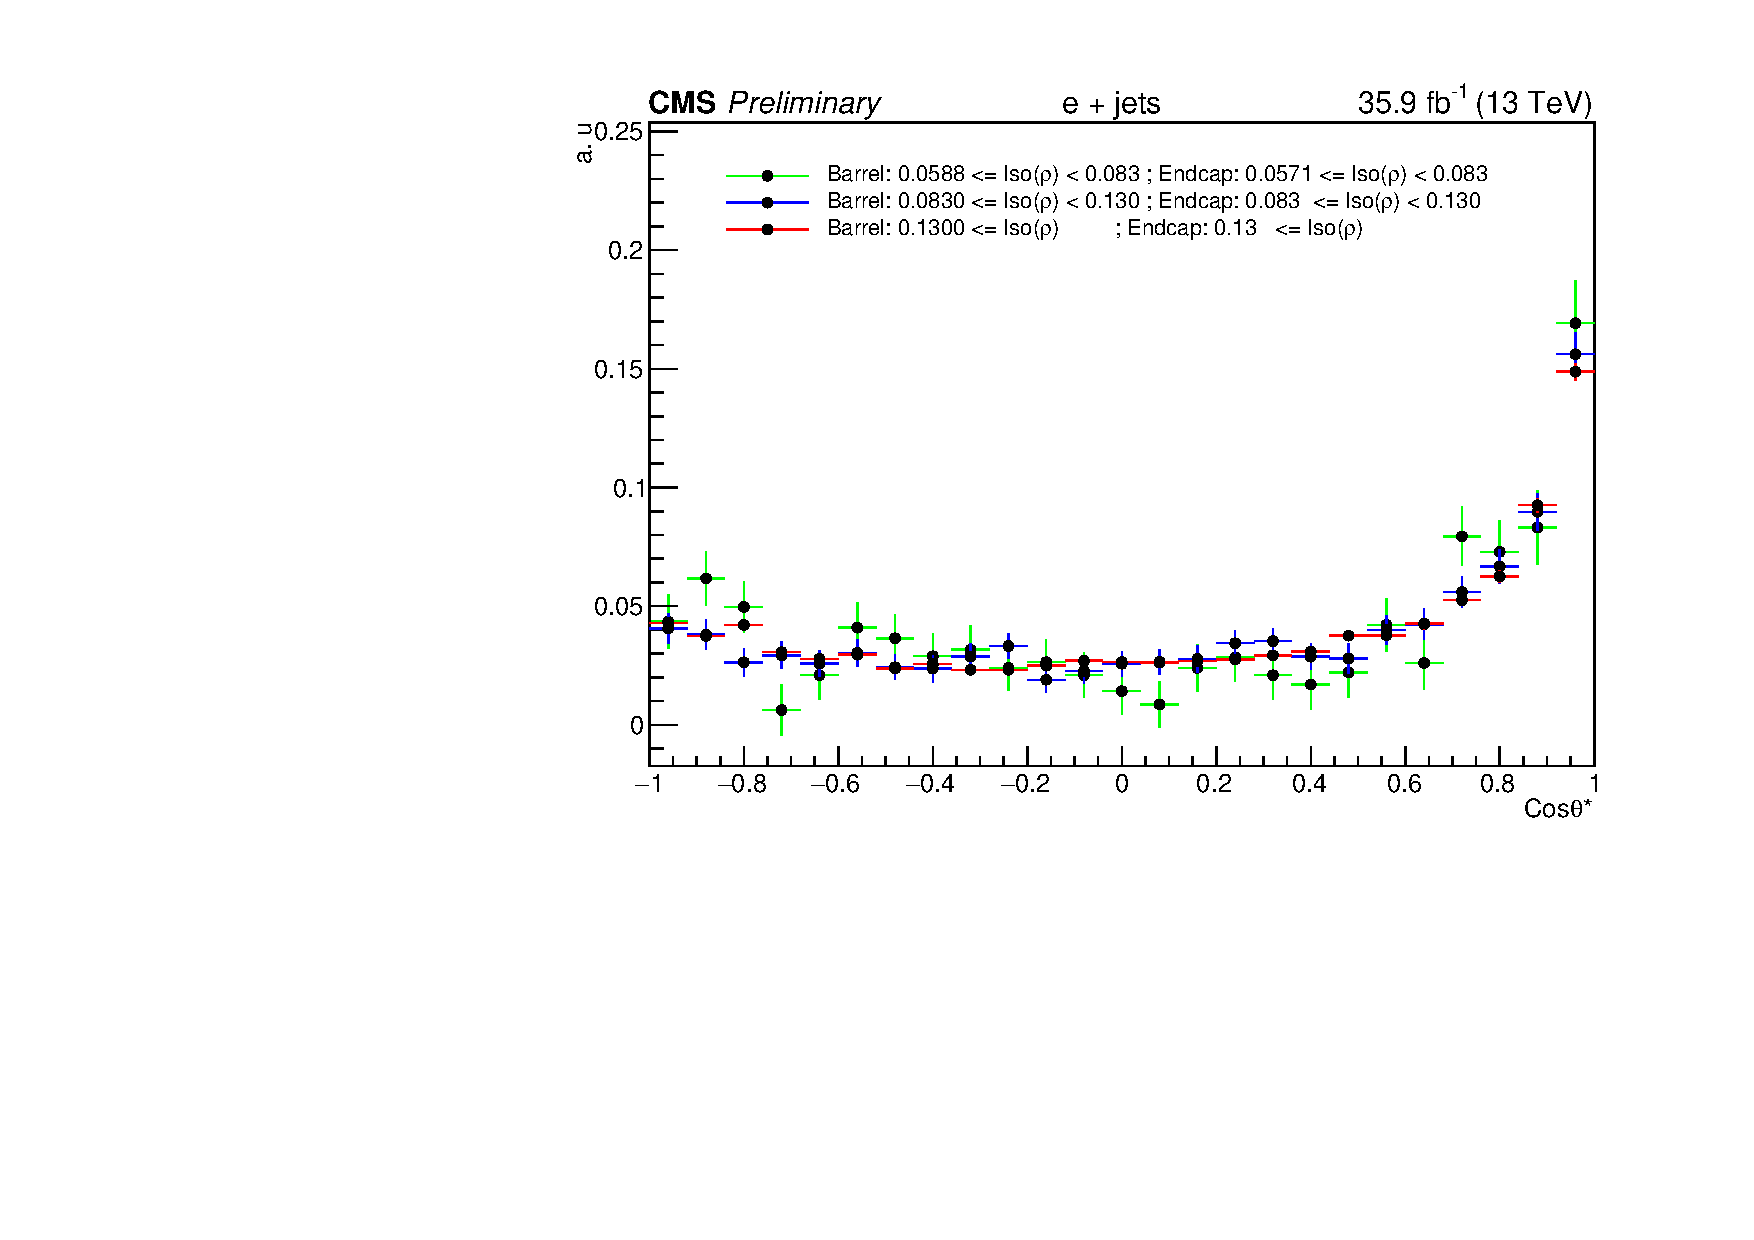
\includegraphics[scale=0.21]{fig/chapt7/qcd/qcd_e_ch/cosine_3region_compare.pdf}
& \hspace{-0.95cm} 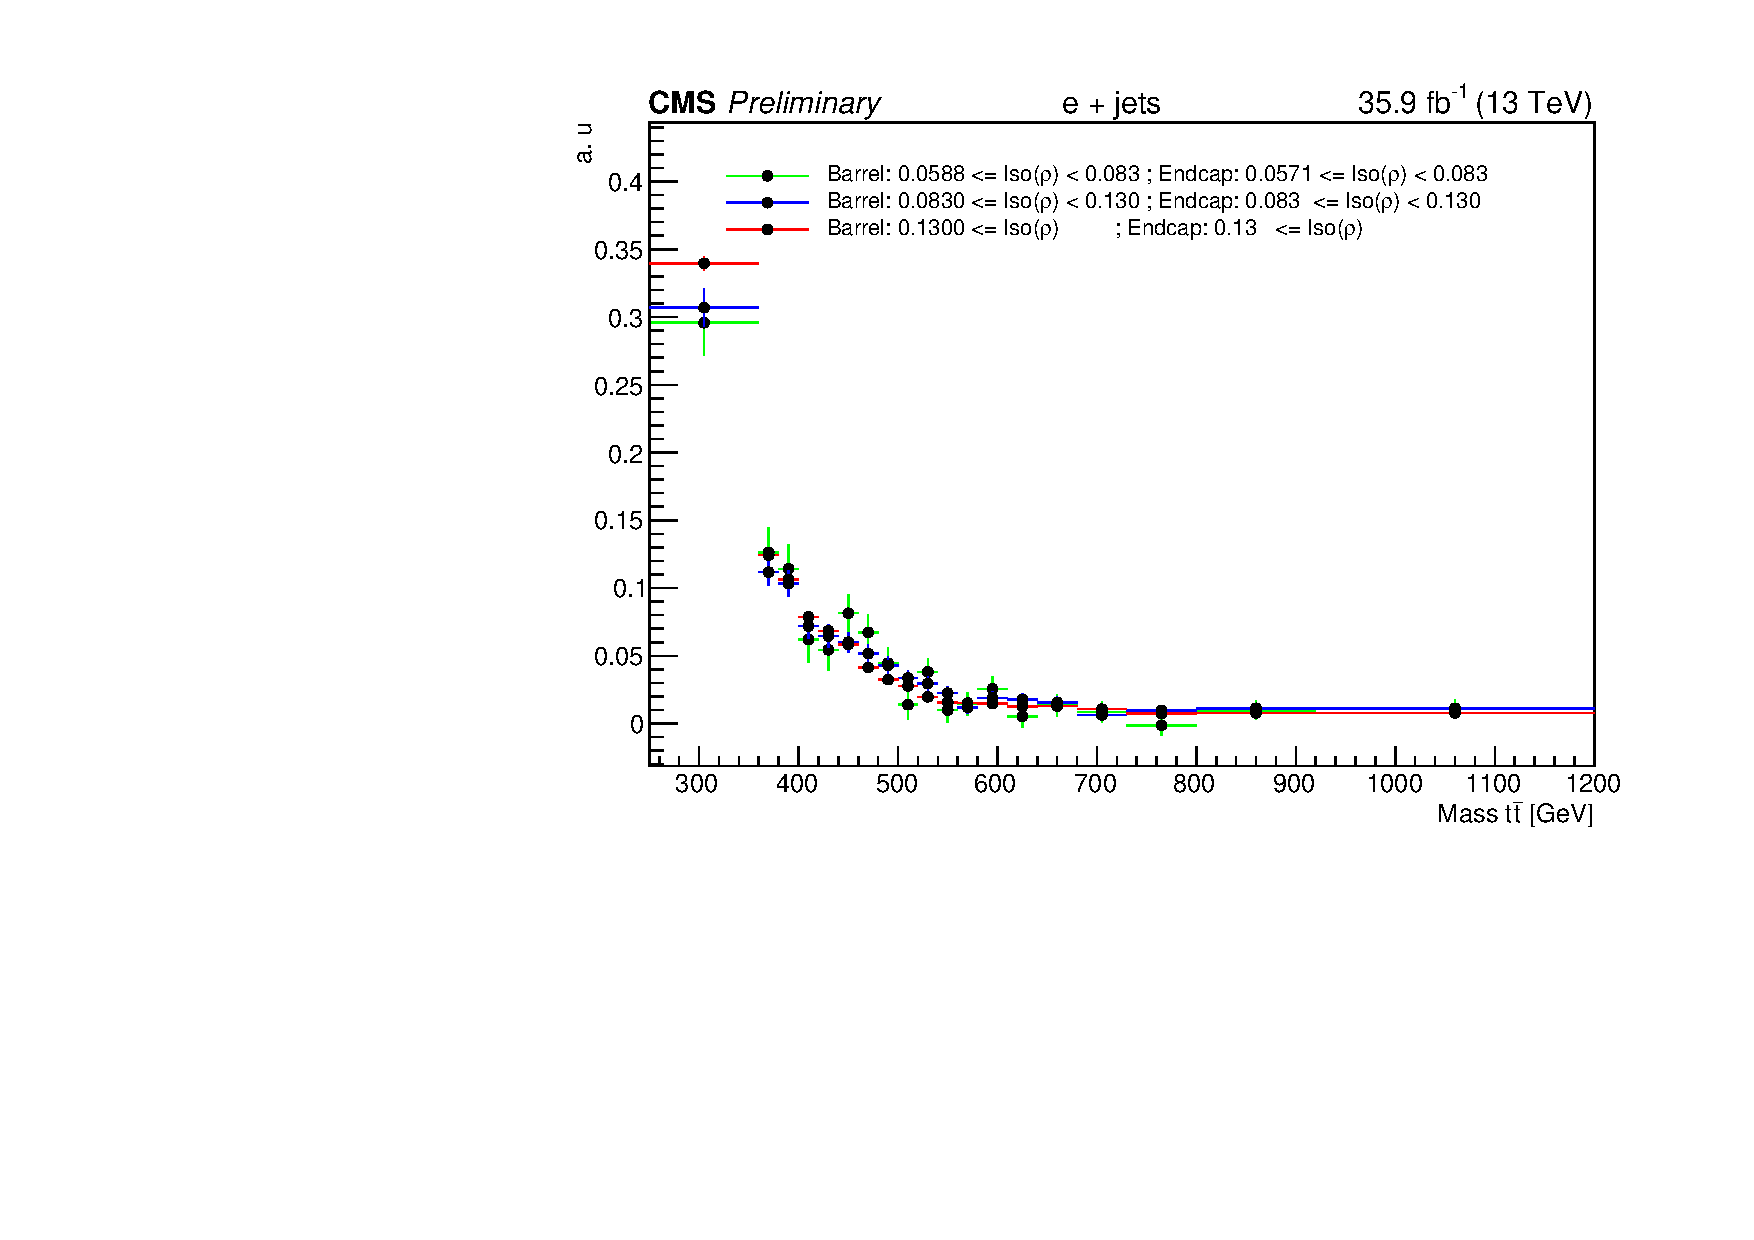
\includegraphics[scale=0.21]{fig/chapt7/qcd/qcd_e_ch/ttbar_m_3region_compare.pdf}\\
($\mathbf{a}$)\qquad\qquad&($\mathbf{b}$)\qquad\qquad&($\mathbf{c}$)\qquad\qquad&($\mathbf{d}$)\qquad\qquad\\ \\
\hspace{-0.5cm}
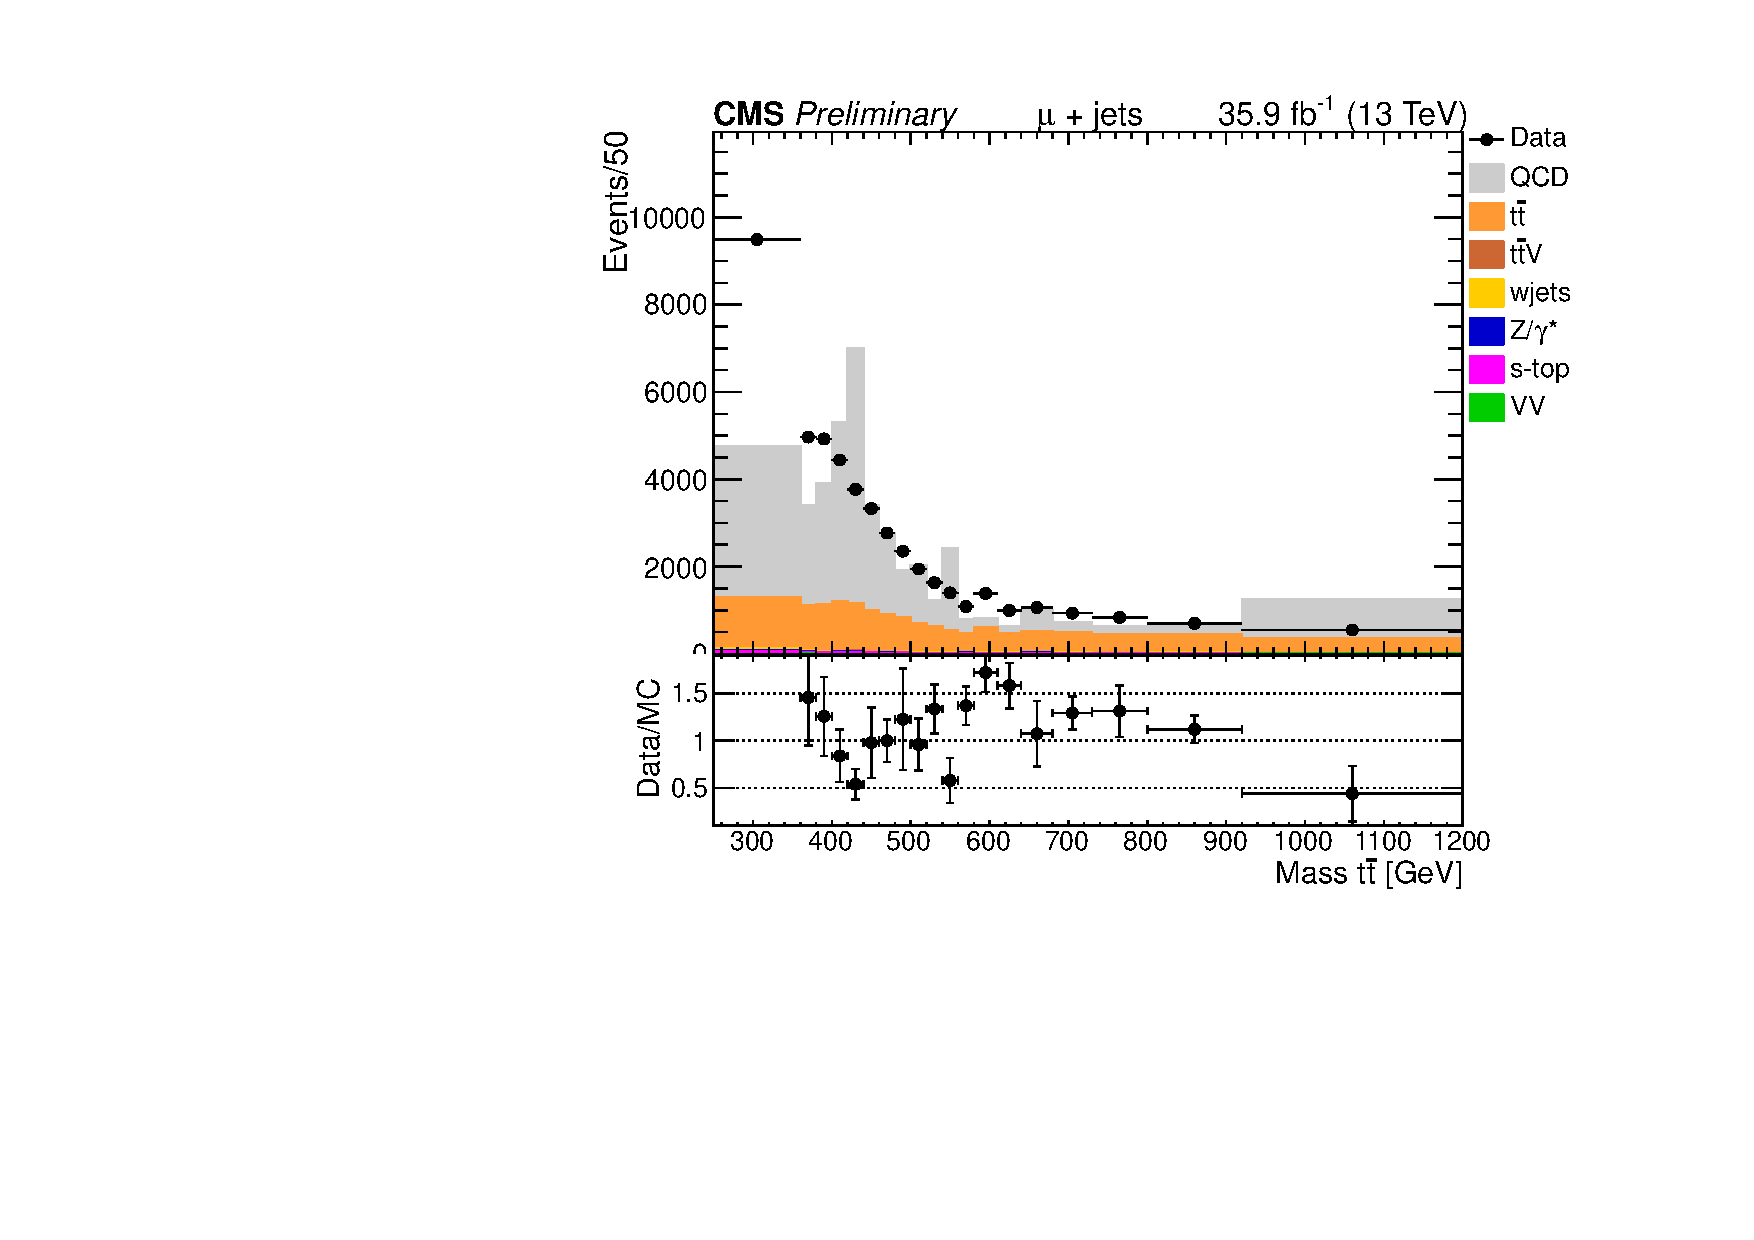
\includegraphics[scale=0.22]{fig/chapt7/qcd/qcd_mu_ch/Mass_H_binned43_Inf.pdf}
& \hspace{-1.0cm} 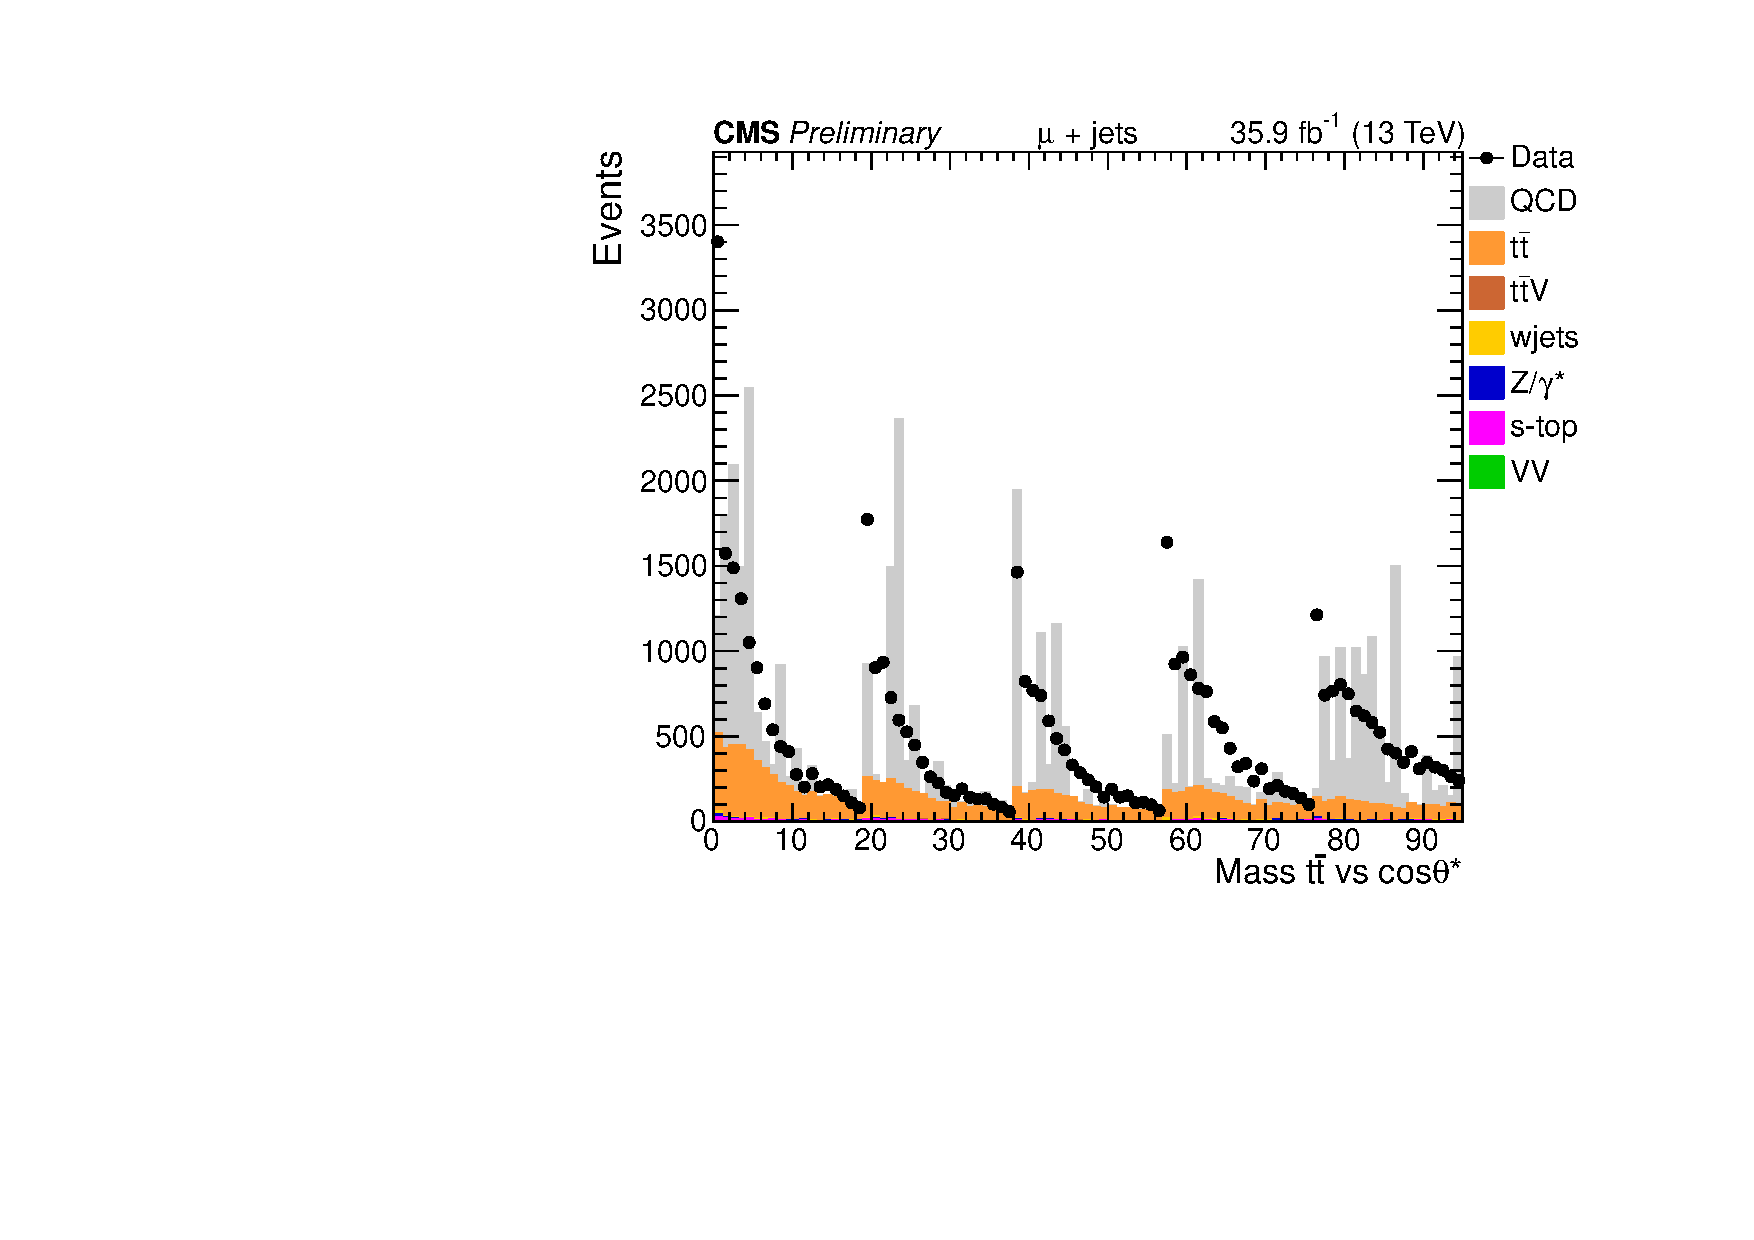
\includegraphics[scale=0.225]{fig/chapt7/qcd/qcd_mu_ch/massH_cos_theta43_Inf.pdf}
& \hspace{-1.0cm} 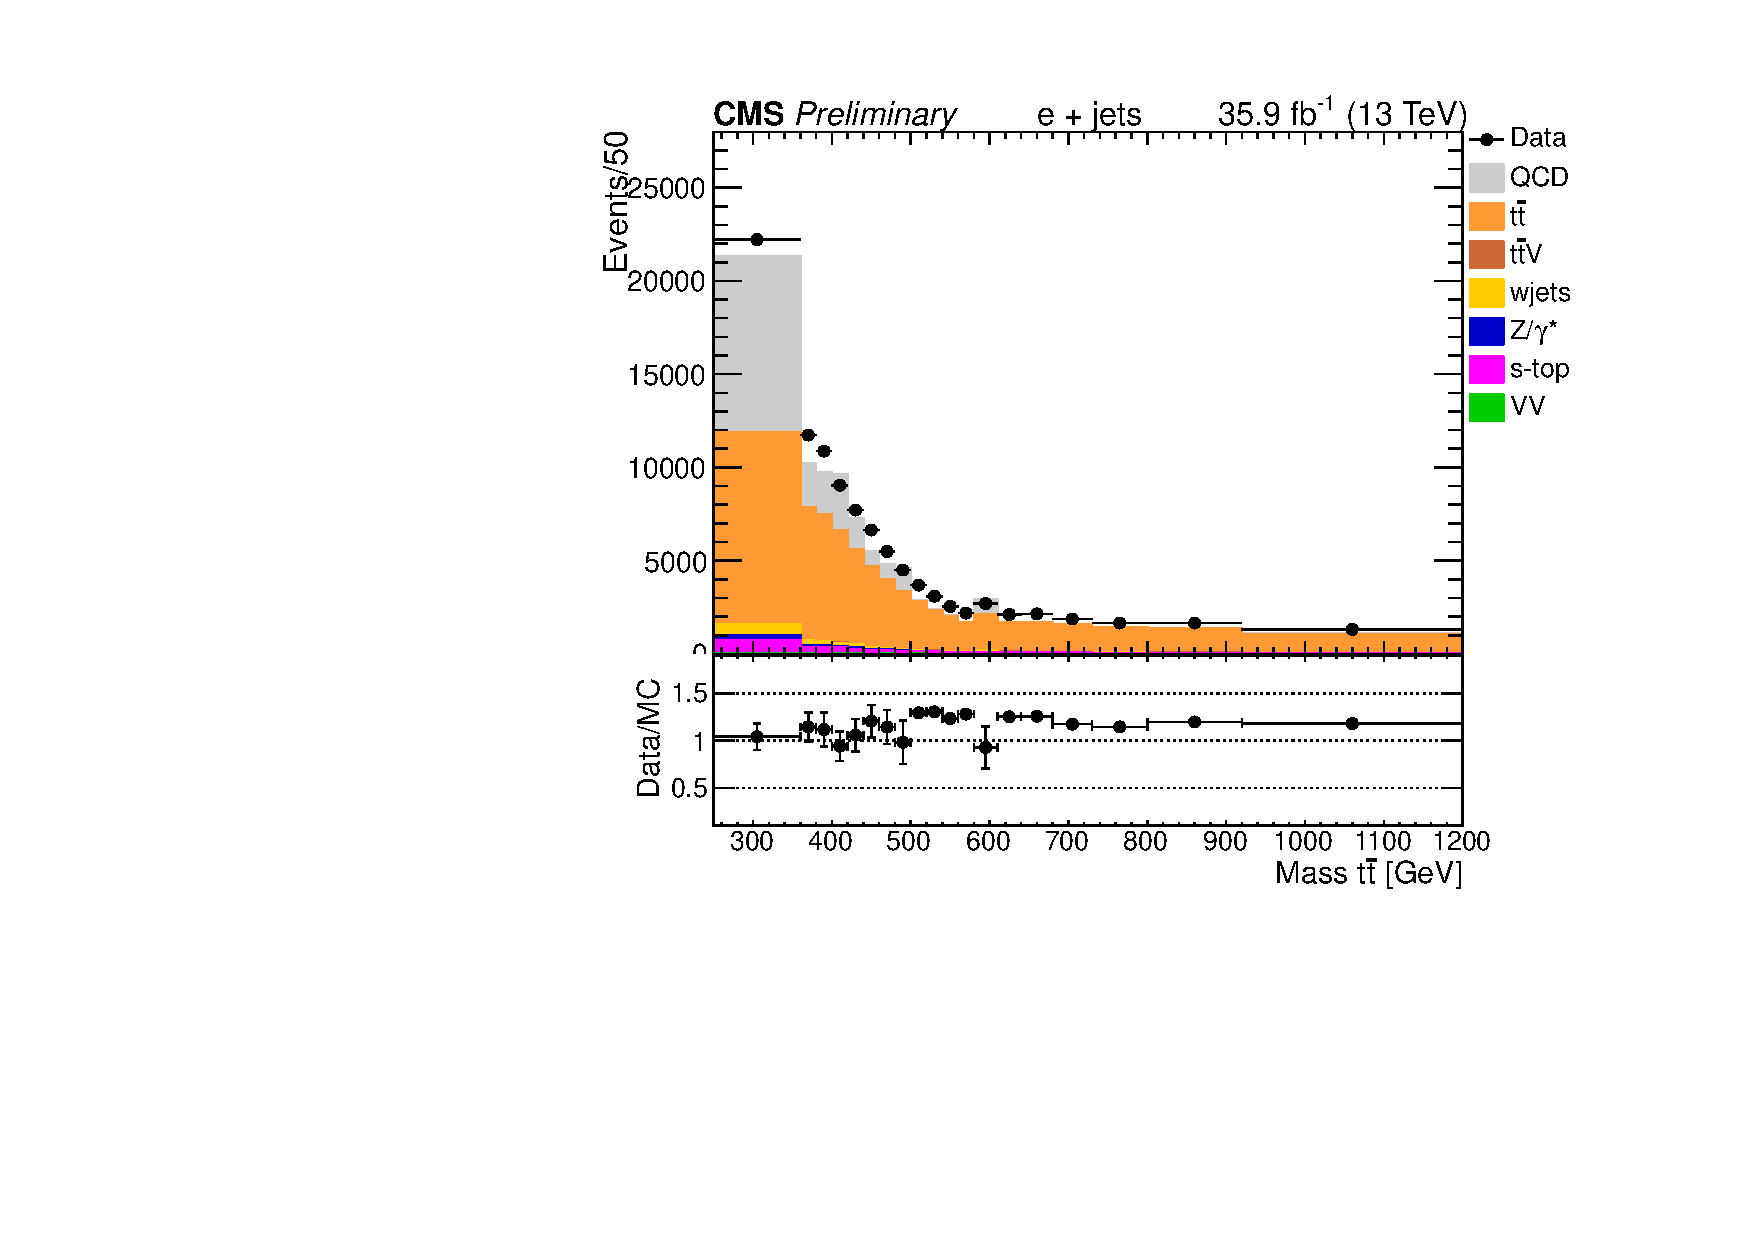
\includegraphics[scale=0.22]{fig/chapt7/qcd/qcd_e_ch/Mass_H_binned_all.pdf}
& \hspace{-1.0cm} 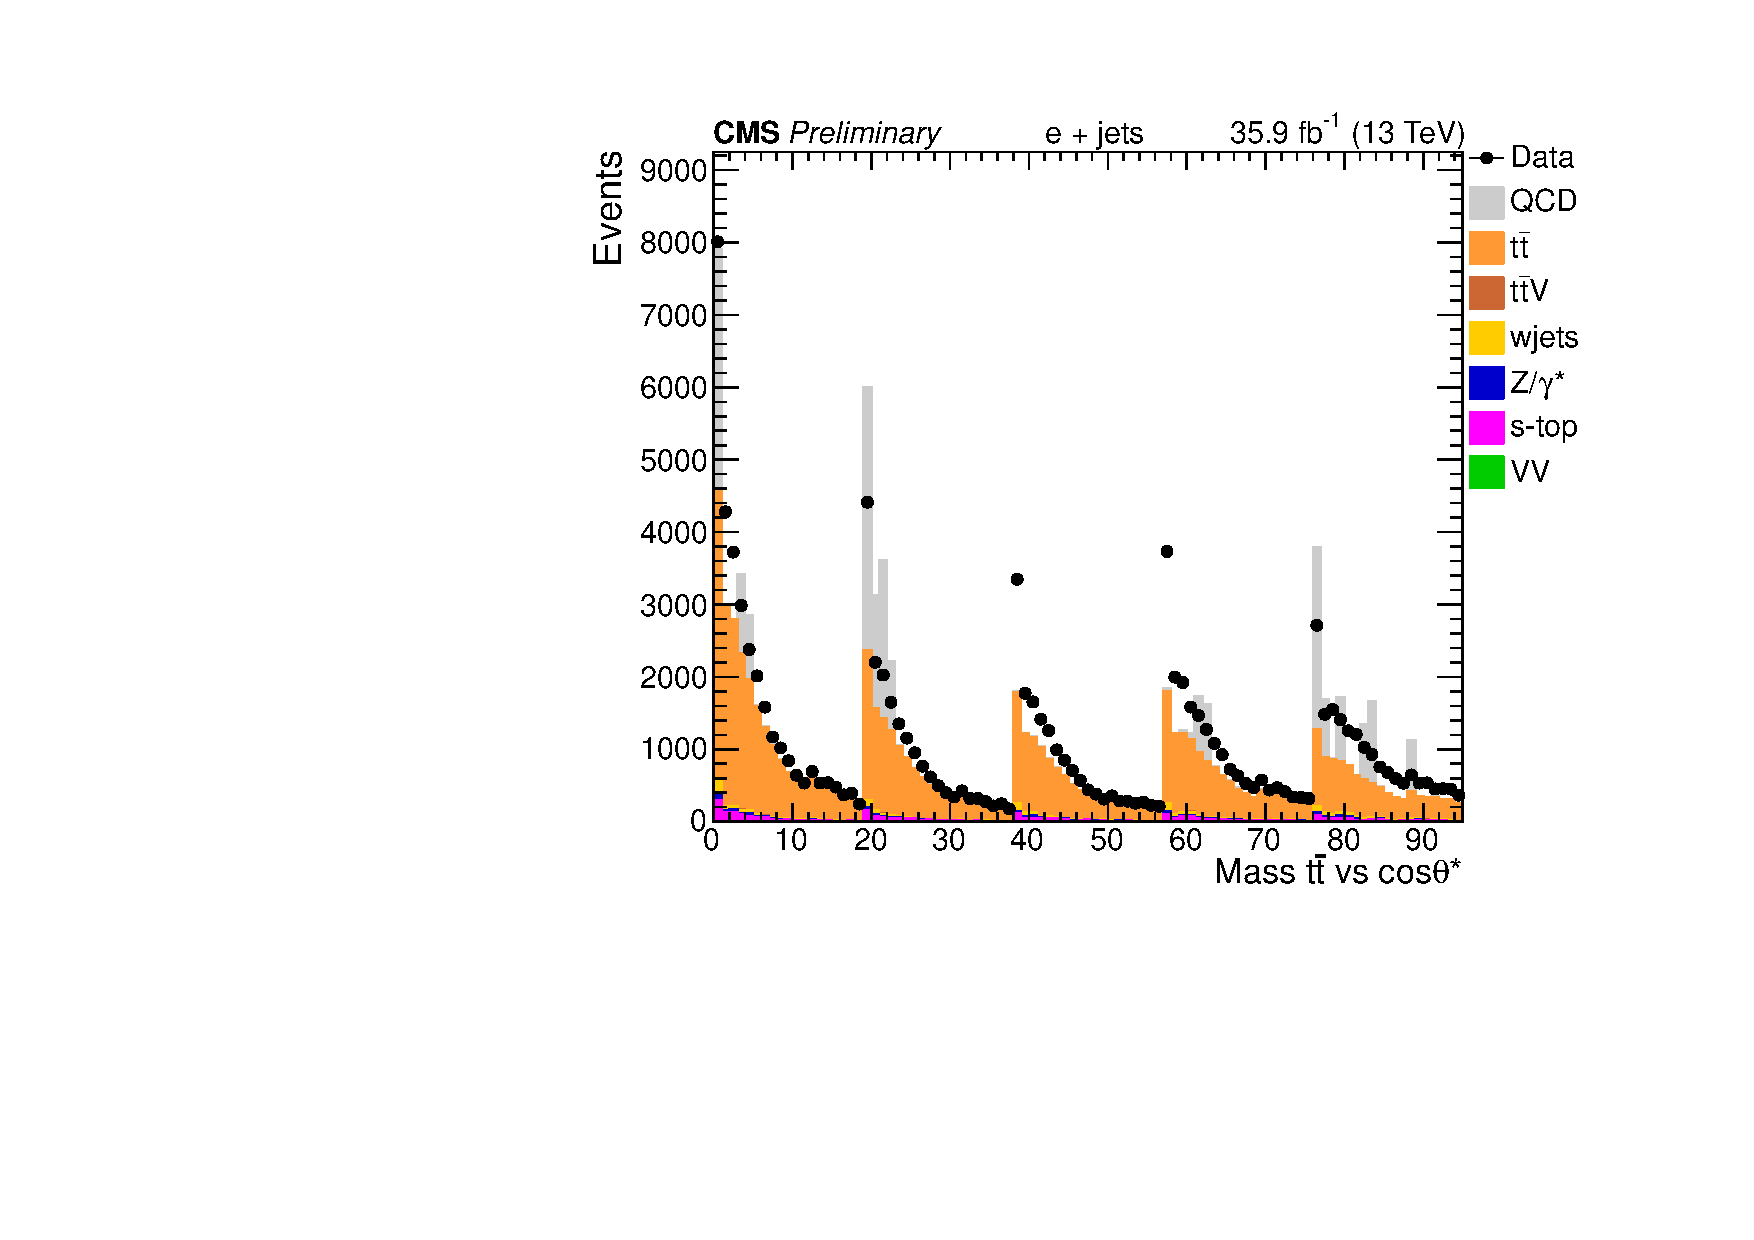
\includegraphics[scale=0.225]{fig/chapt7/qcd/qcd_e_ch/massH_cos_theta_all.pdf}\\
($\mathbf{e}$)\qquad\qquad&($\mathbf{f}$)\qquad\qquad&($\mathbf{g}$)\qquad\qquad&($\mathbf{h}$)\qquad\qquad\\
\\
\hspace{-0.5cm}
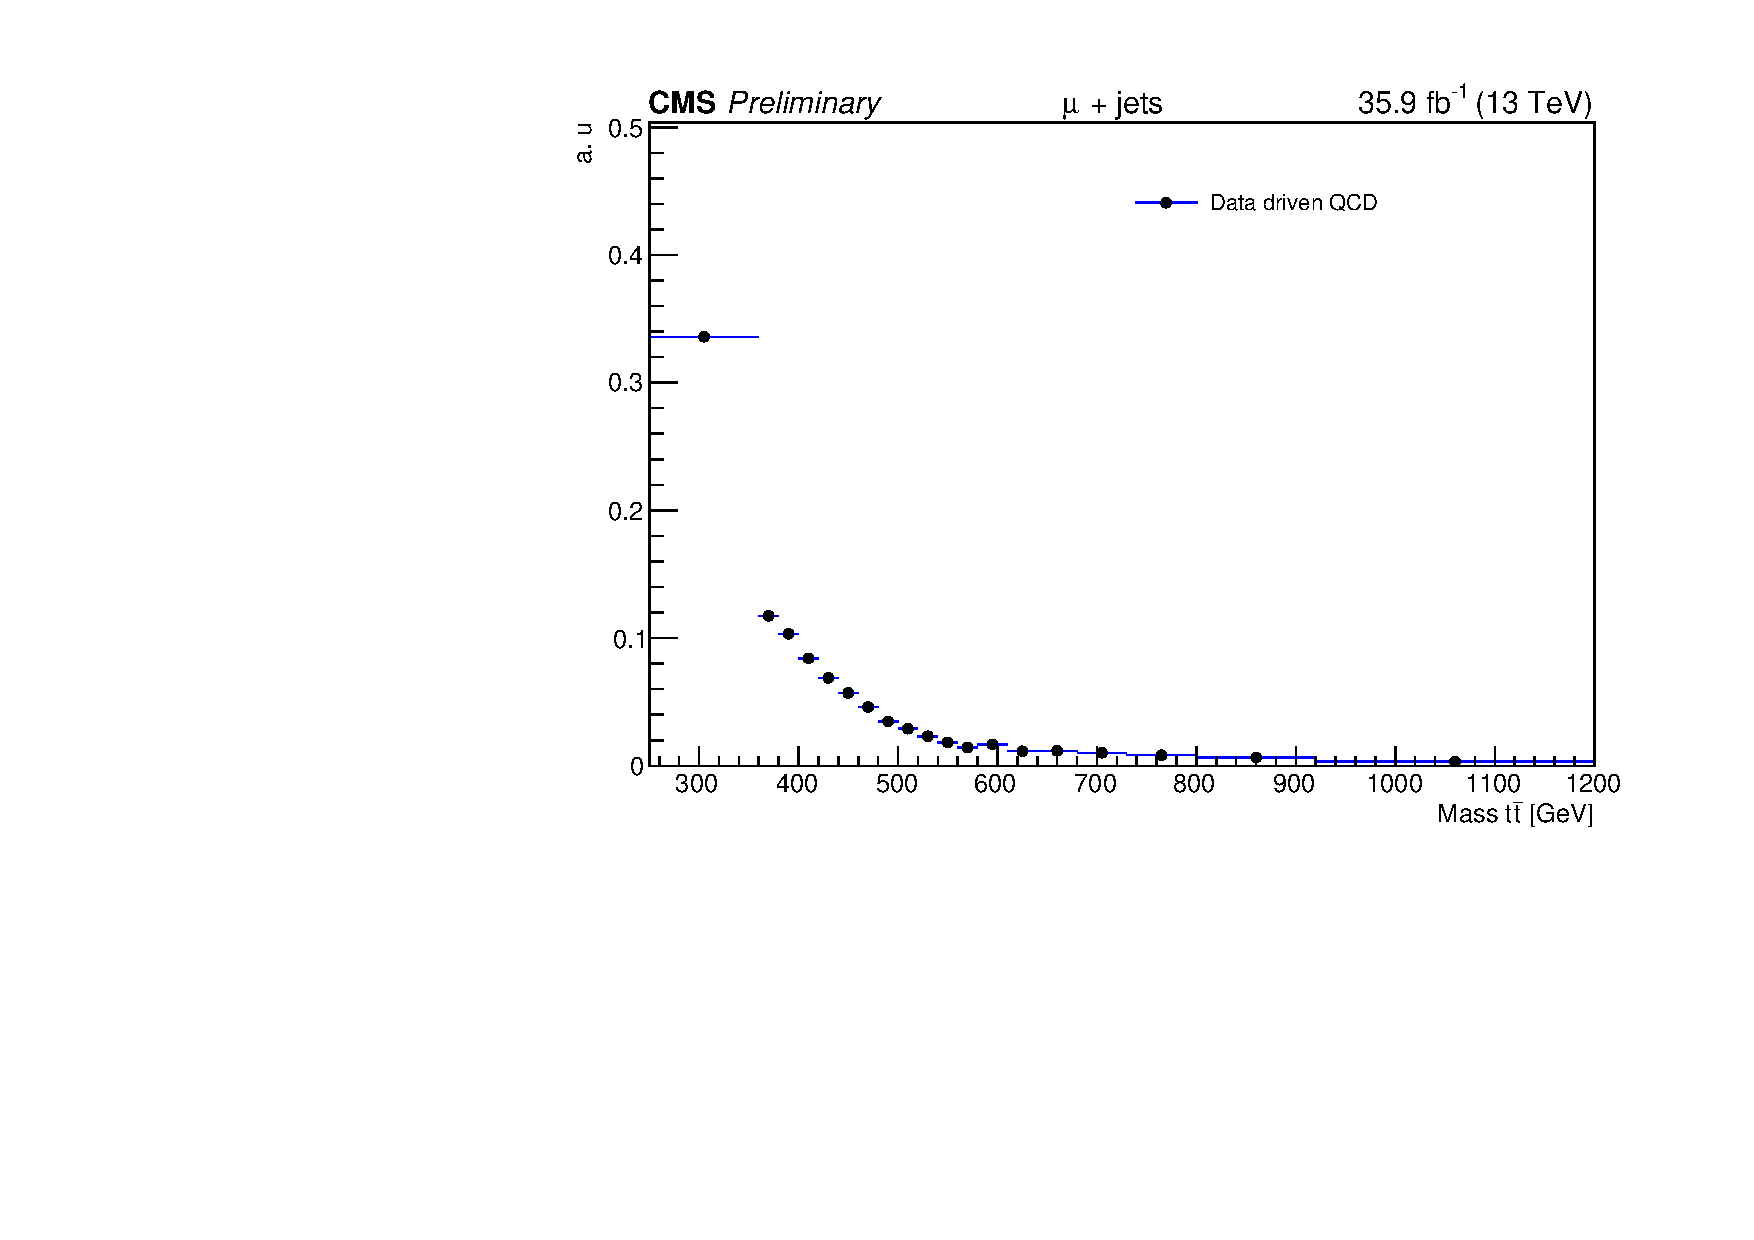
\includegraphics[scale=0.22]{fig/chapt7/qcd/qcd_mu_ch/ttbar_m_data_drivenQCD.pdf}
& \hspace{-0.95cm} 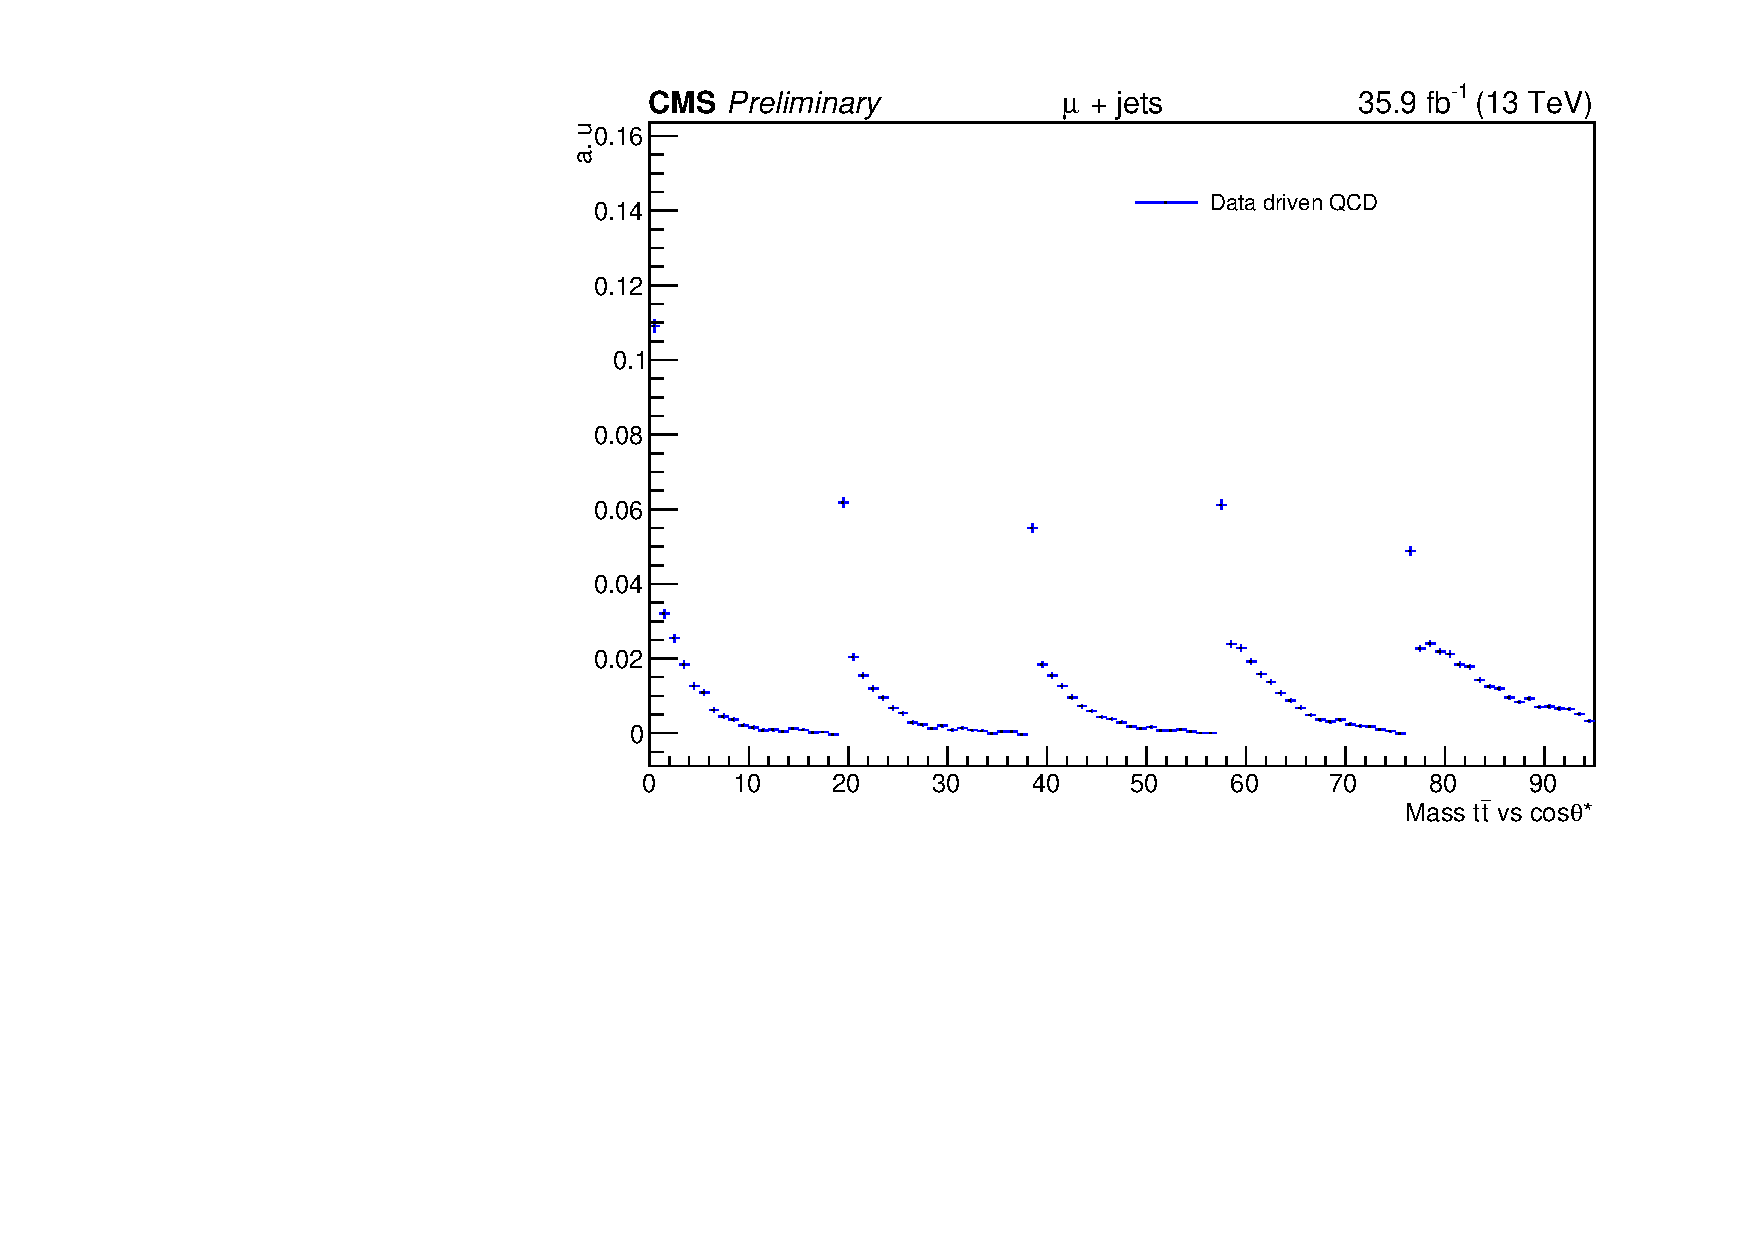
\includegraphics[scale=0.22]{fig/chapt7/qcd/qcd_mu_ch/ttbar_m_cos_data_drivenQCD.pdf}
& \hspace{-0.95cm} 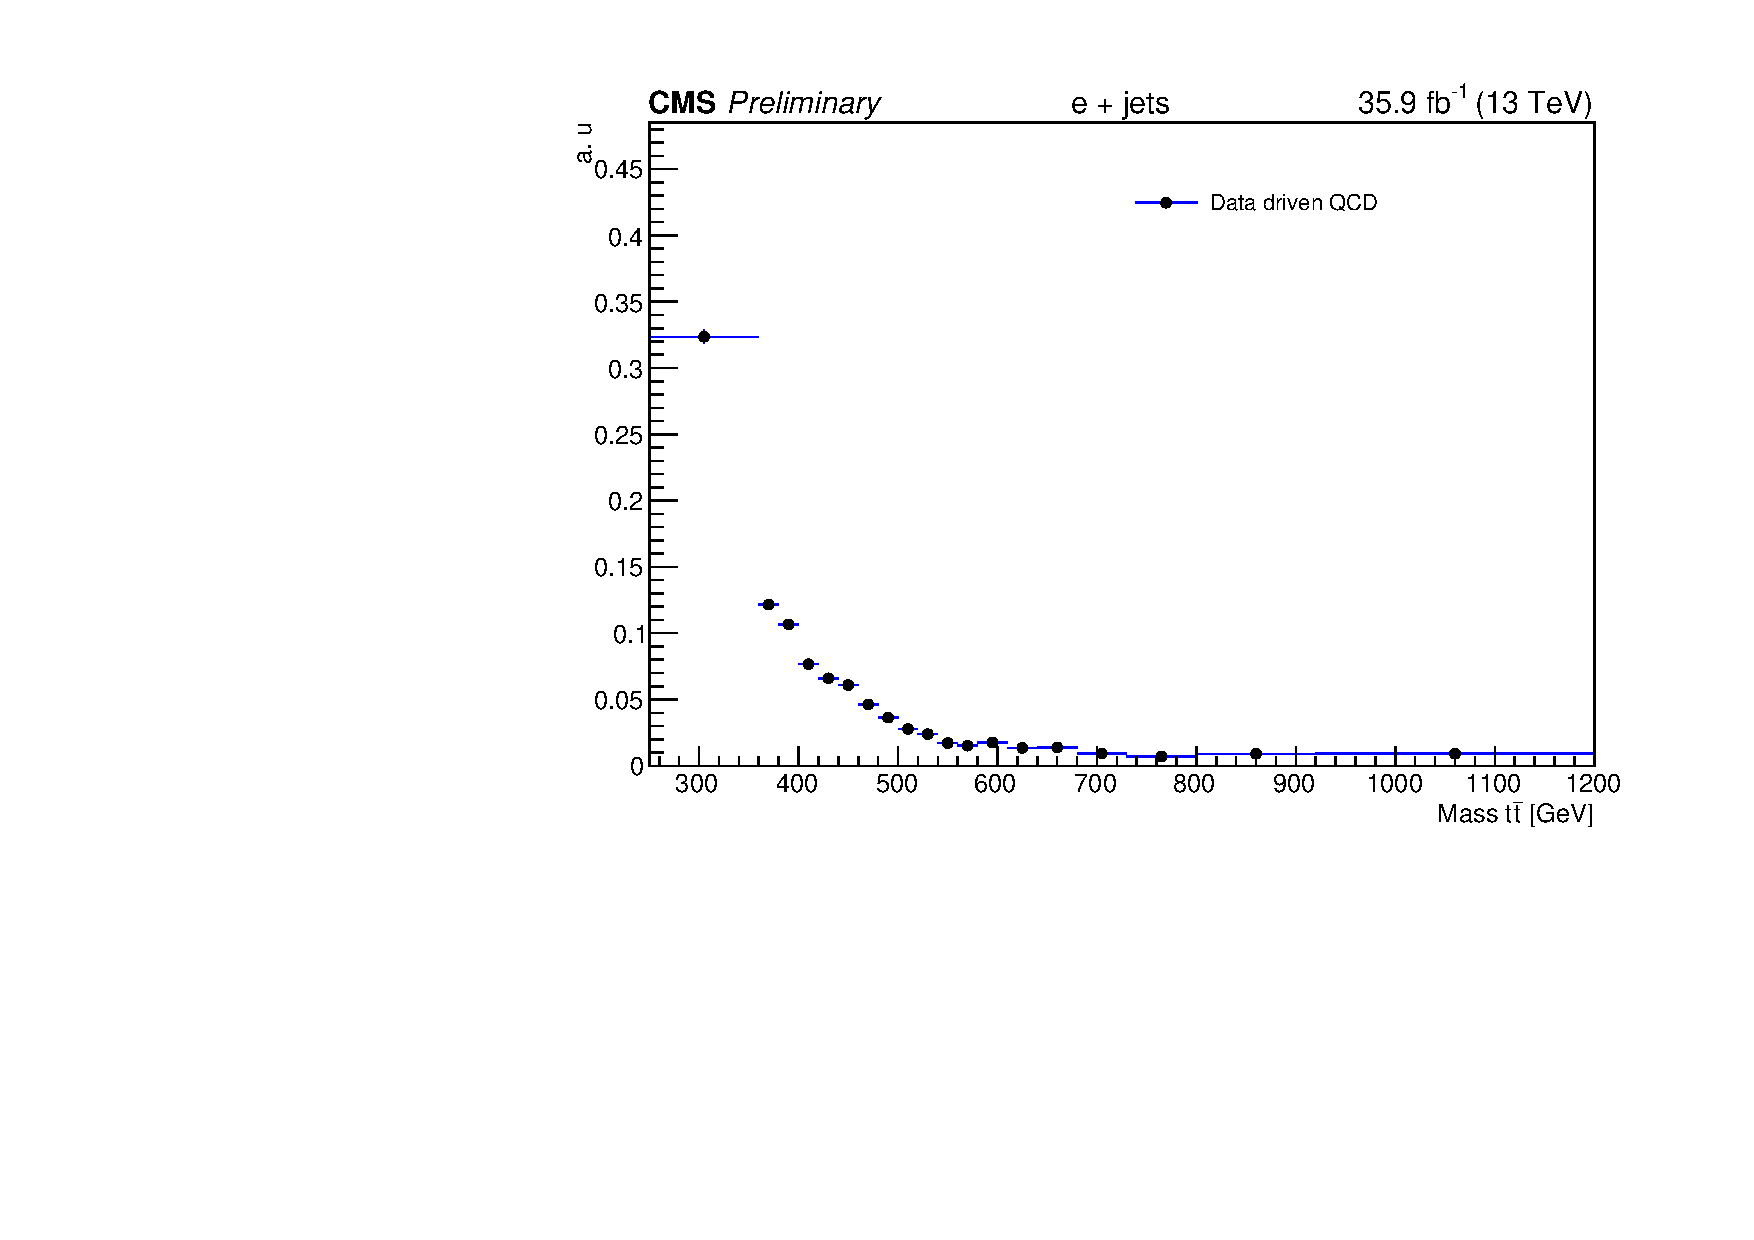
\includegraphics[scale=0.22]{fig/chapt7/qcd/qcd_e_ch/ttbar_m_data_drivenQCD.pdf}
& \hspace{-0.95cm} 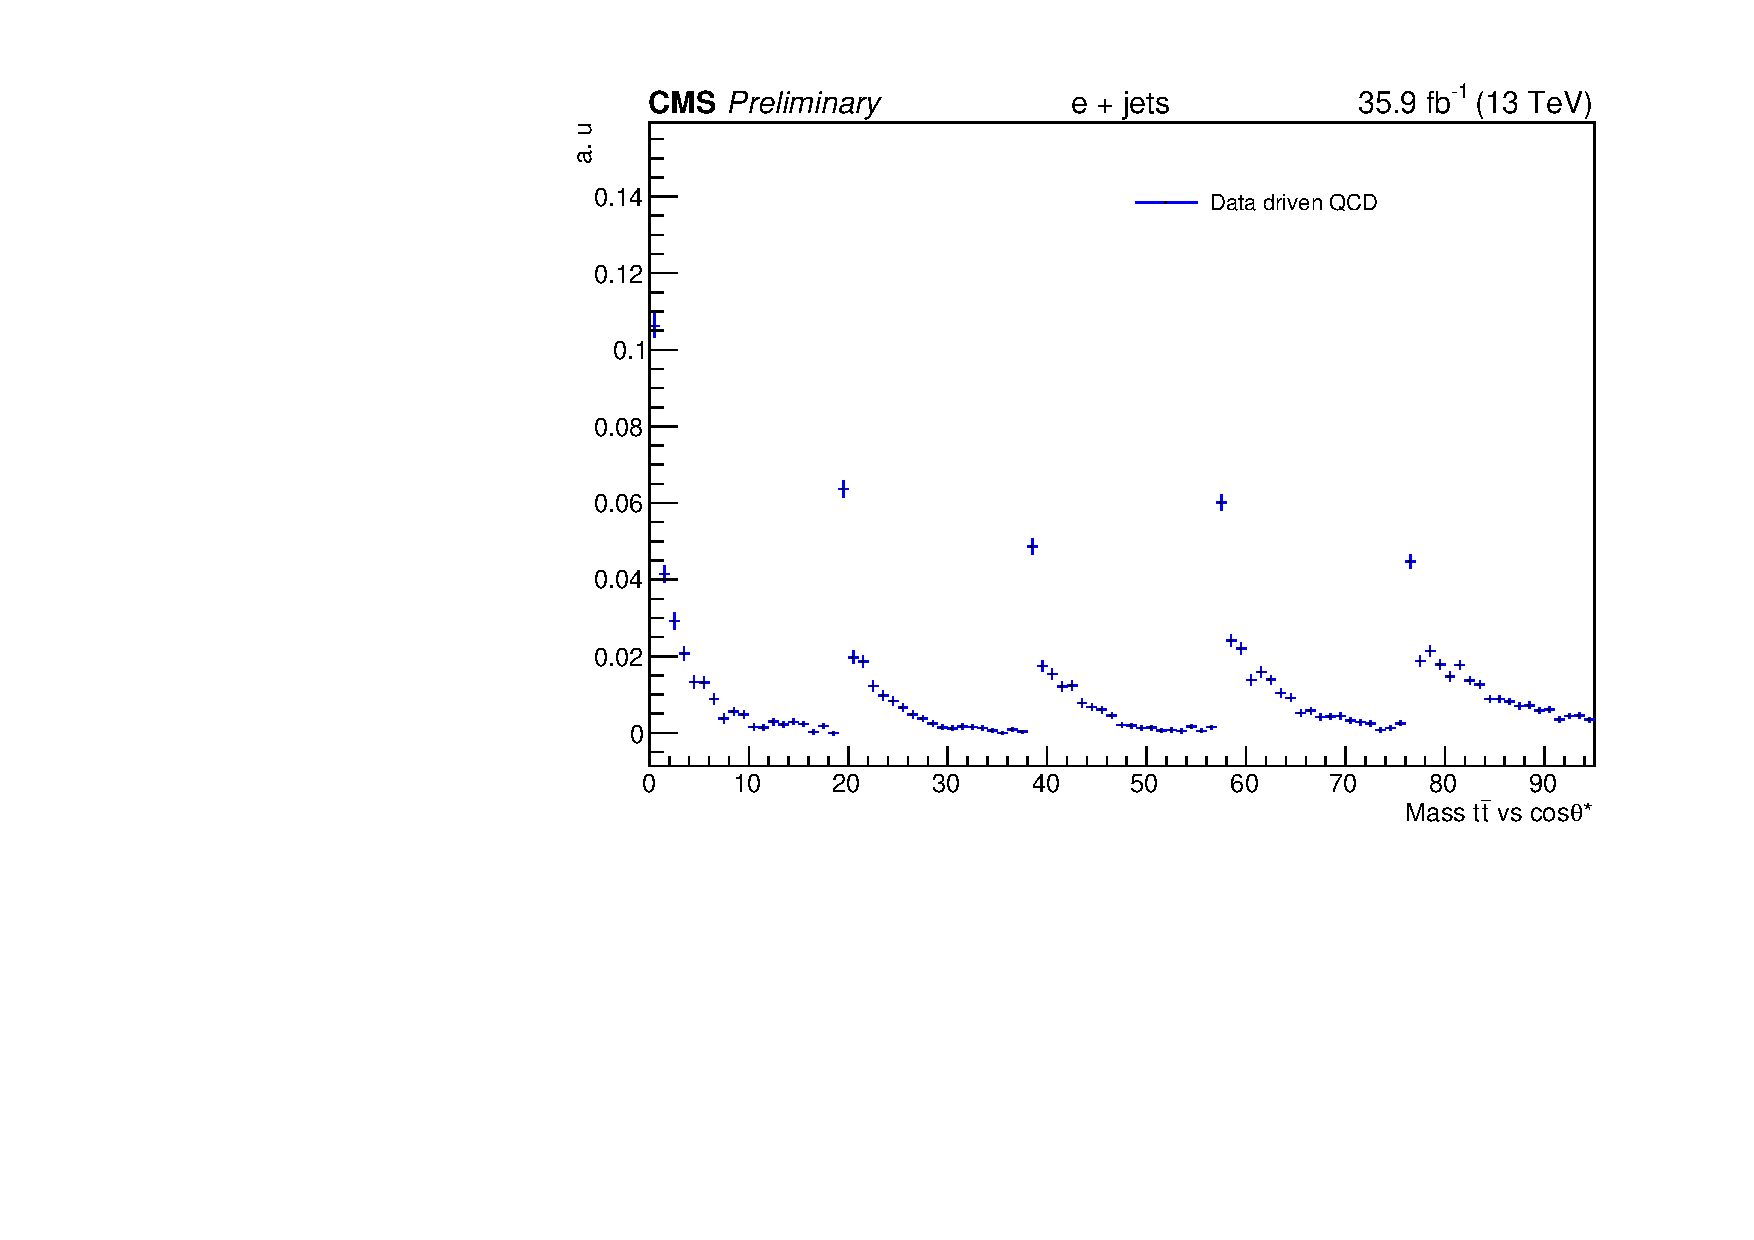
\includegraphics[scale=0.22]{fig/chapt7/qcd/qcd_e_ch/ttbar_m_cos_data_drivenQCD.pdf}\\
($\mathbf{i}$)\qquad\qquad&($\mathbf{j}$)\qquad\qquad&($\mathbf{k}$)\qquad\qquad&($\mathbf{l}$)\qquad\qquad\\
\\
\hspace{-0.5cm}
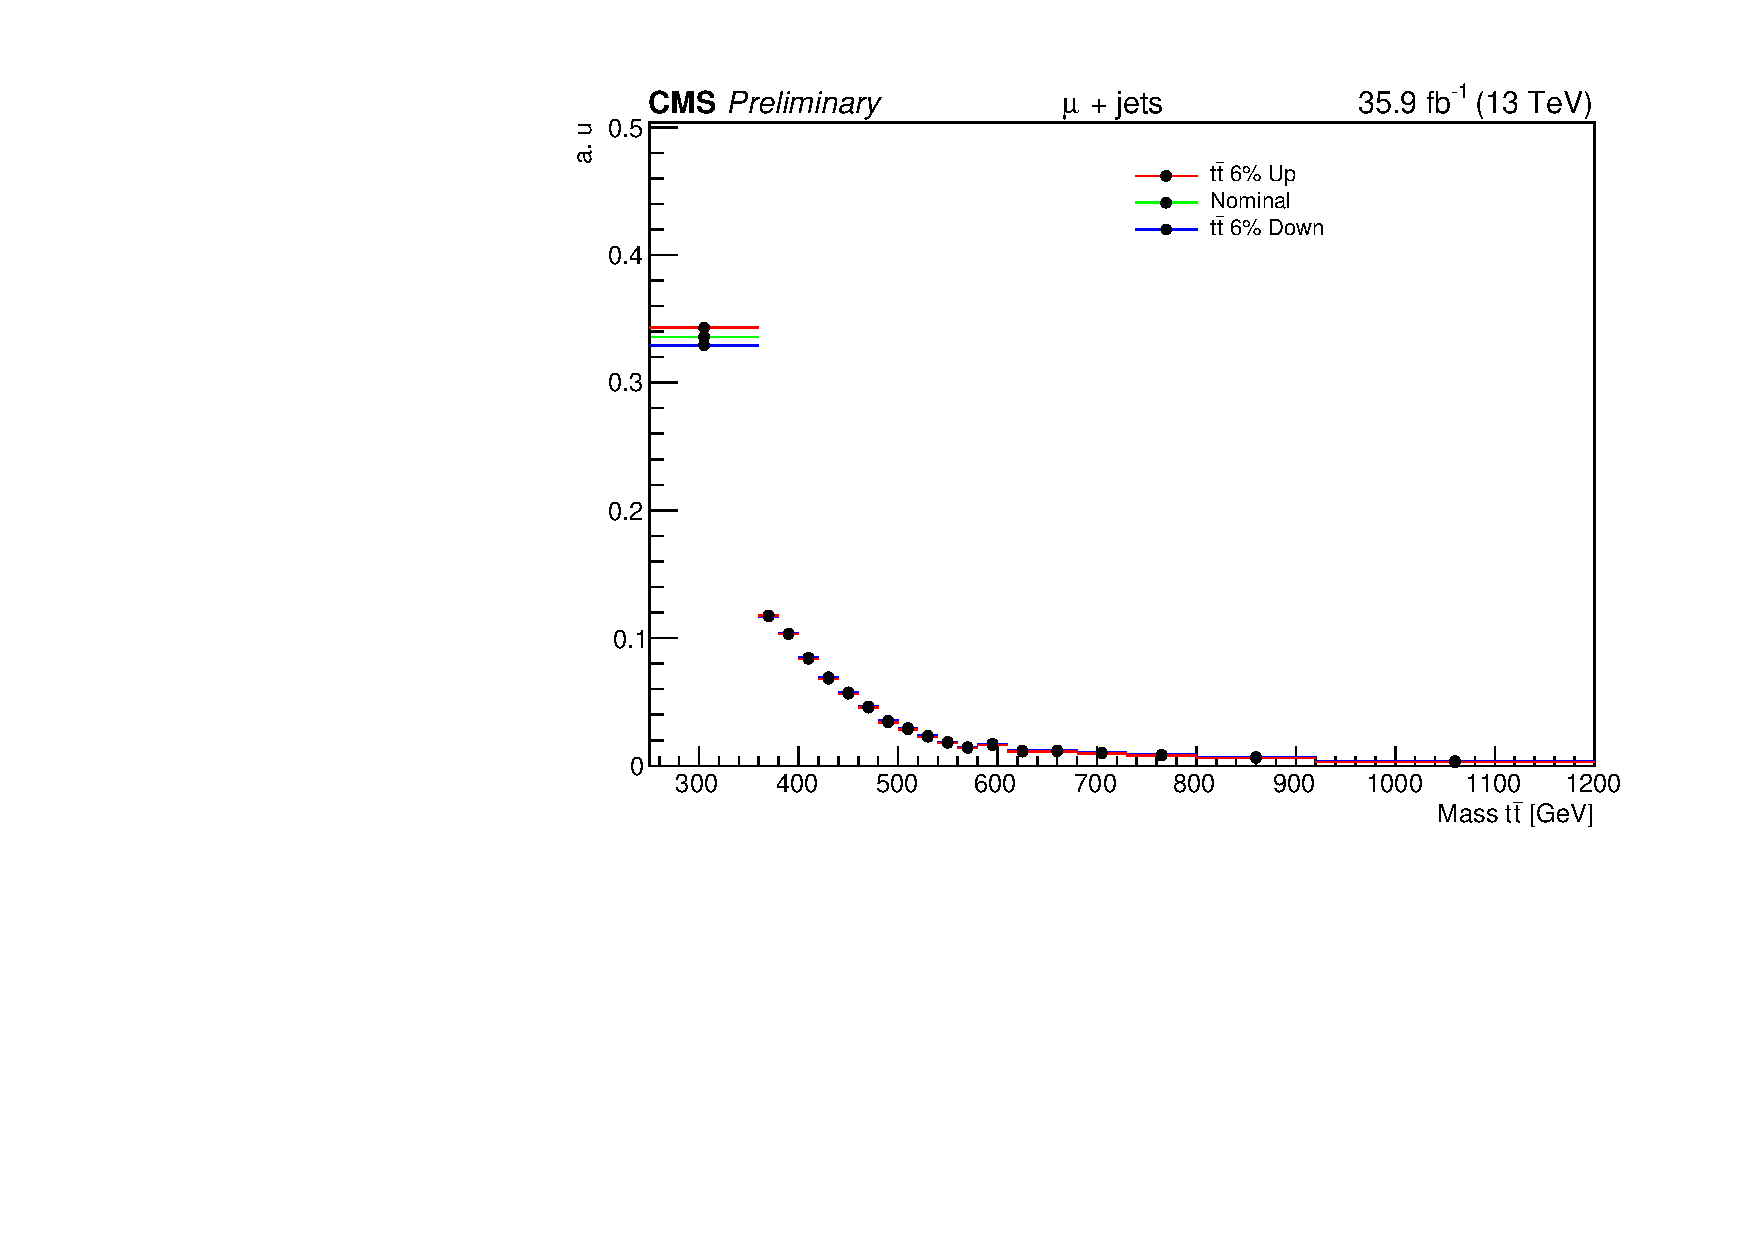
\includegraphics[scale=0.22]{fig/chapt7/qcd/qcd_mu_ch/ttbar_m_ttsys_UpDn.pdf}
& \hspace{-0.95cm} 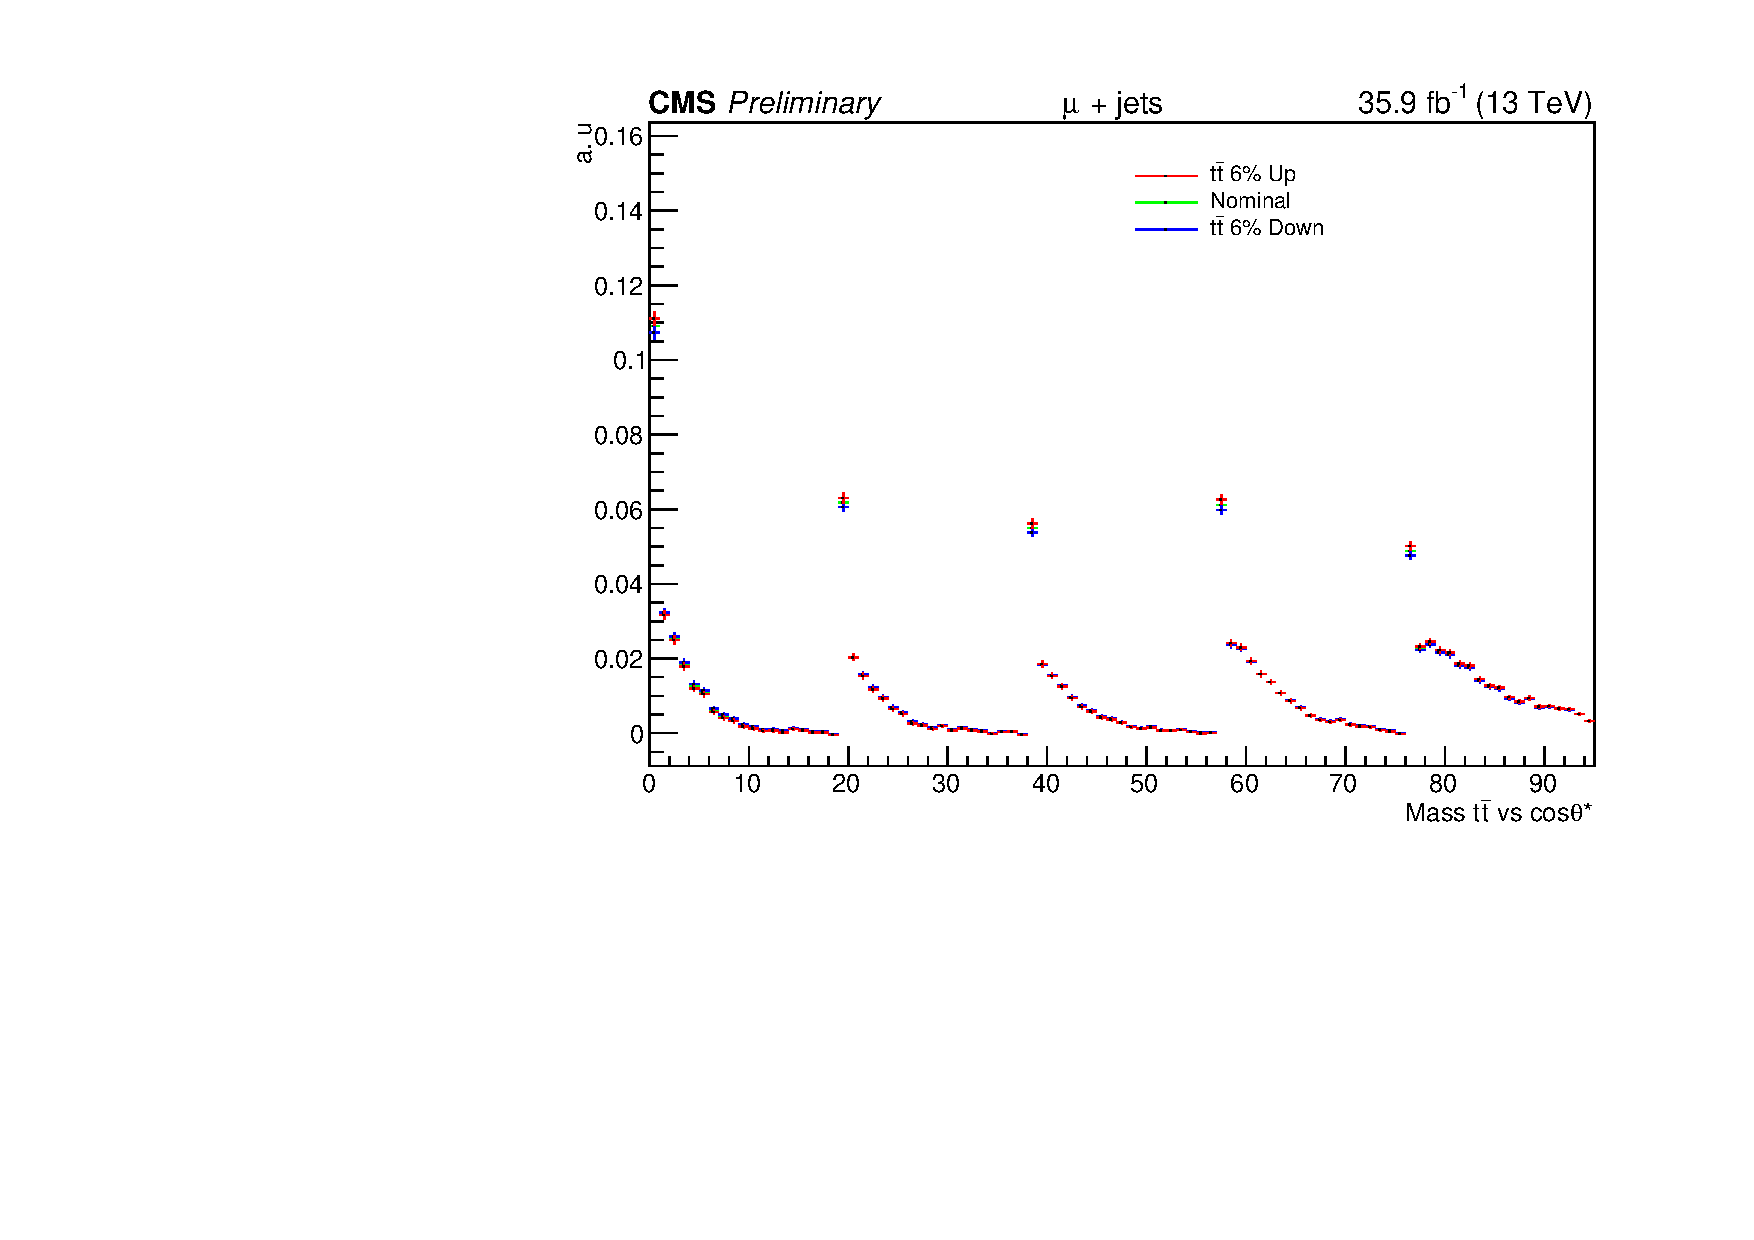
\includegraphics[scale=0.22]{fig/chapt7/qcd/qcd_mu_ch/ttbar_m_cosine_ttsysUpDn.pdf}
& \hspace{-0.95cm} 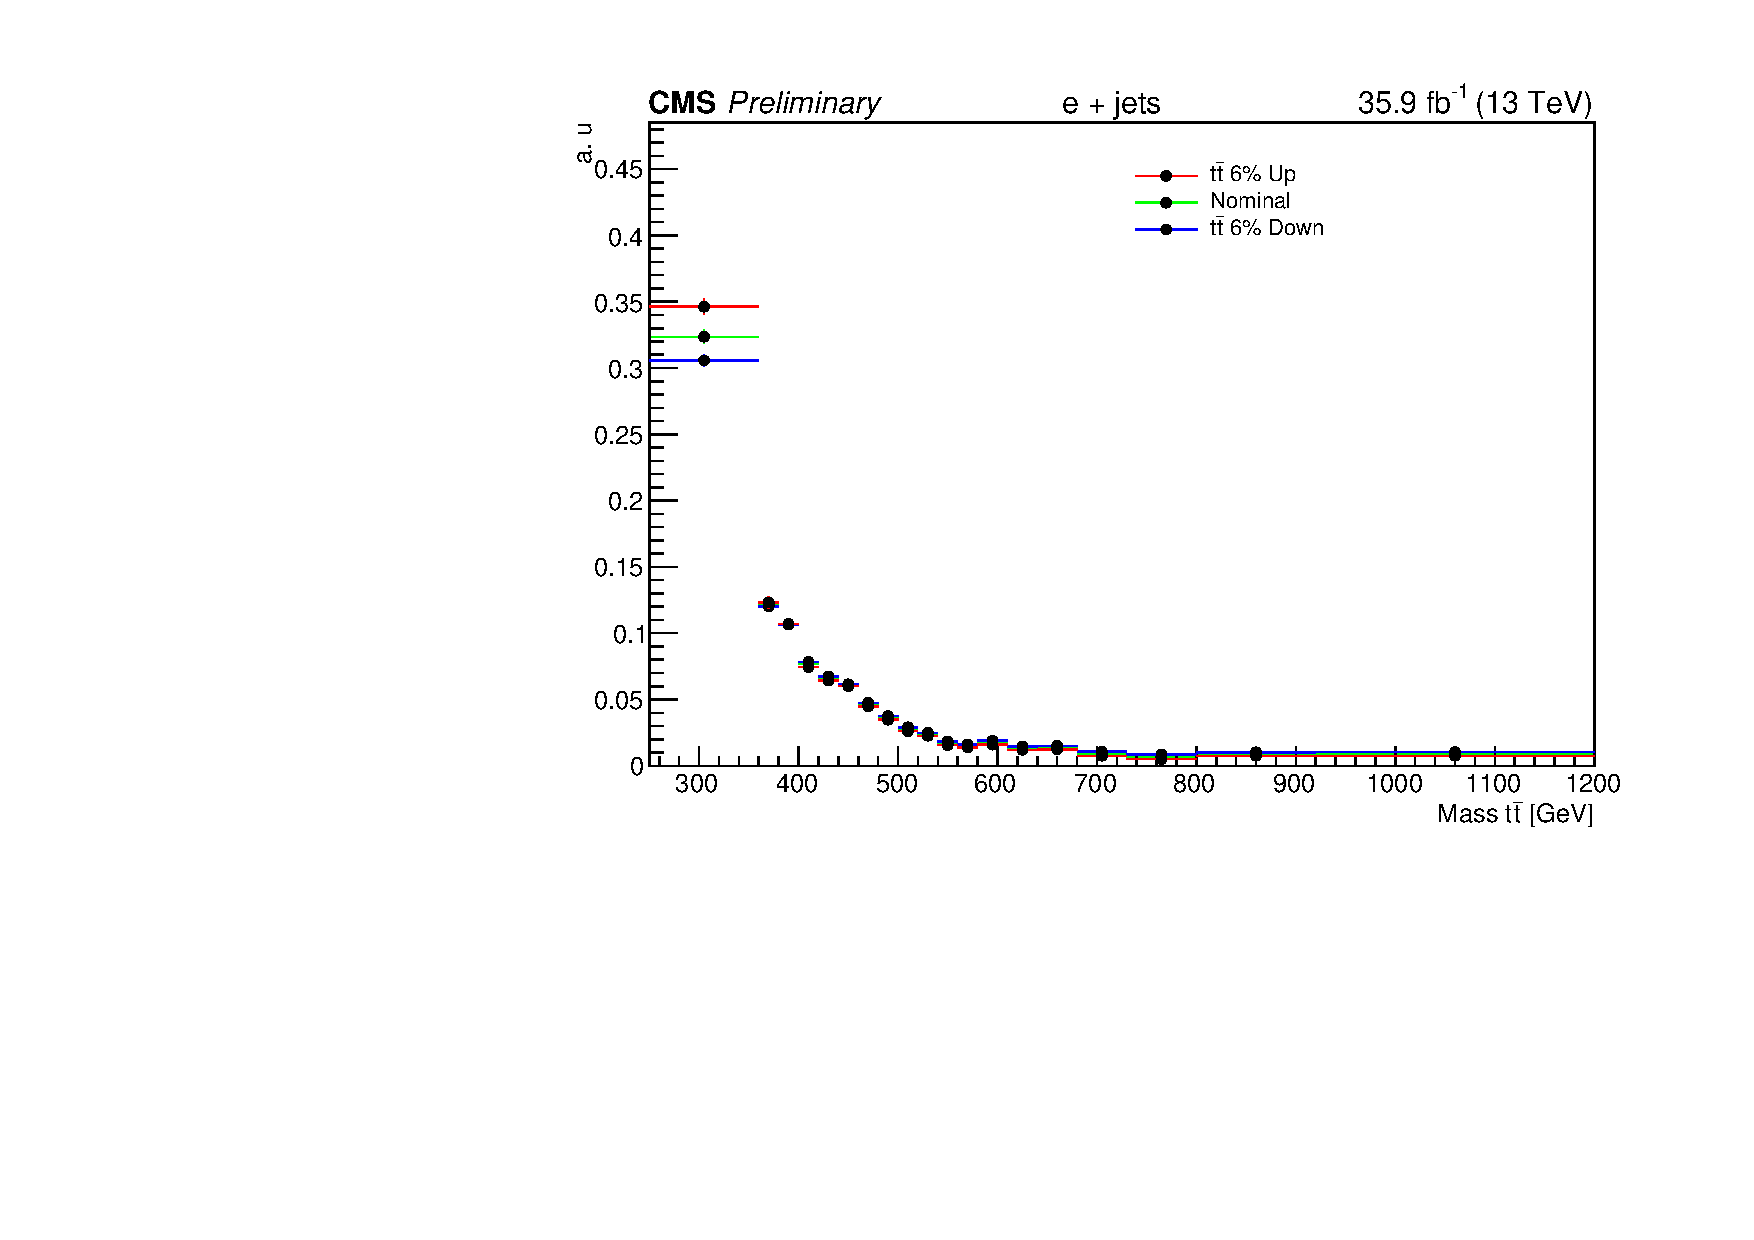
\includegraphics[scale=0.22]{fig/chapt7/qcd/qcd_e_ch/ttbar_m_ttsys_6perUpDn.pdf}
& \hspace{-0.95cm} 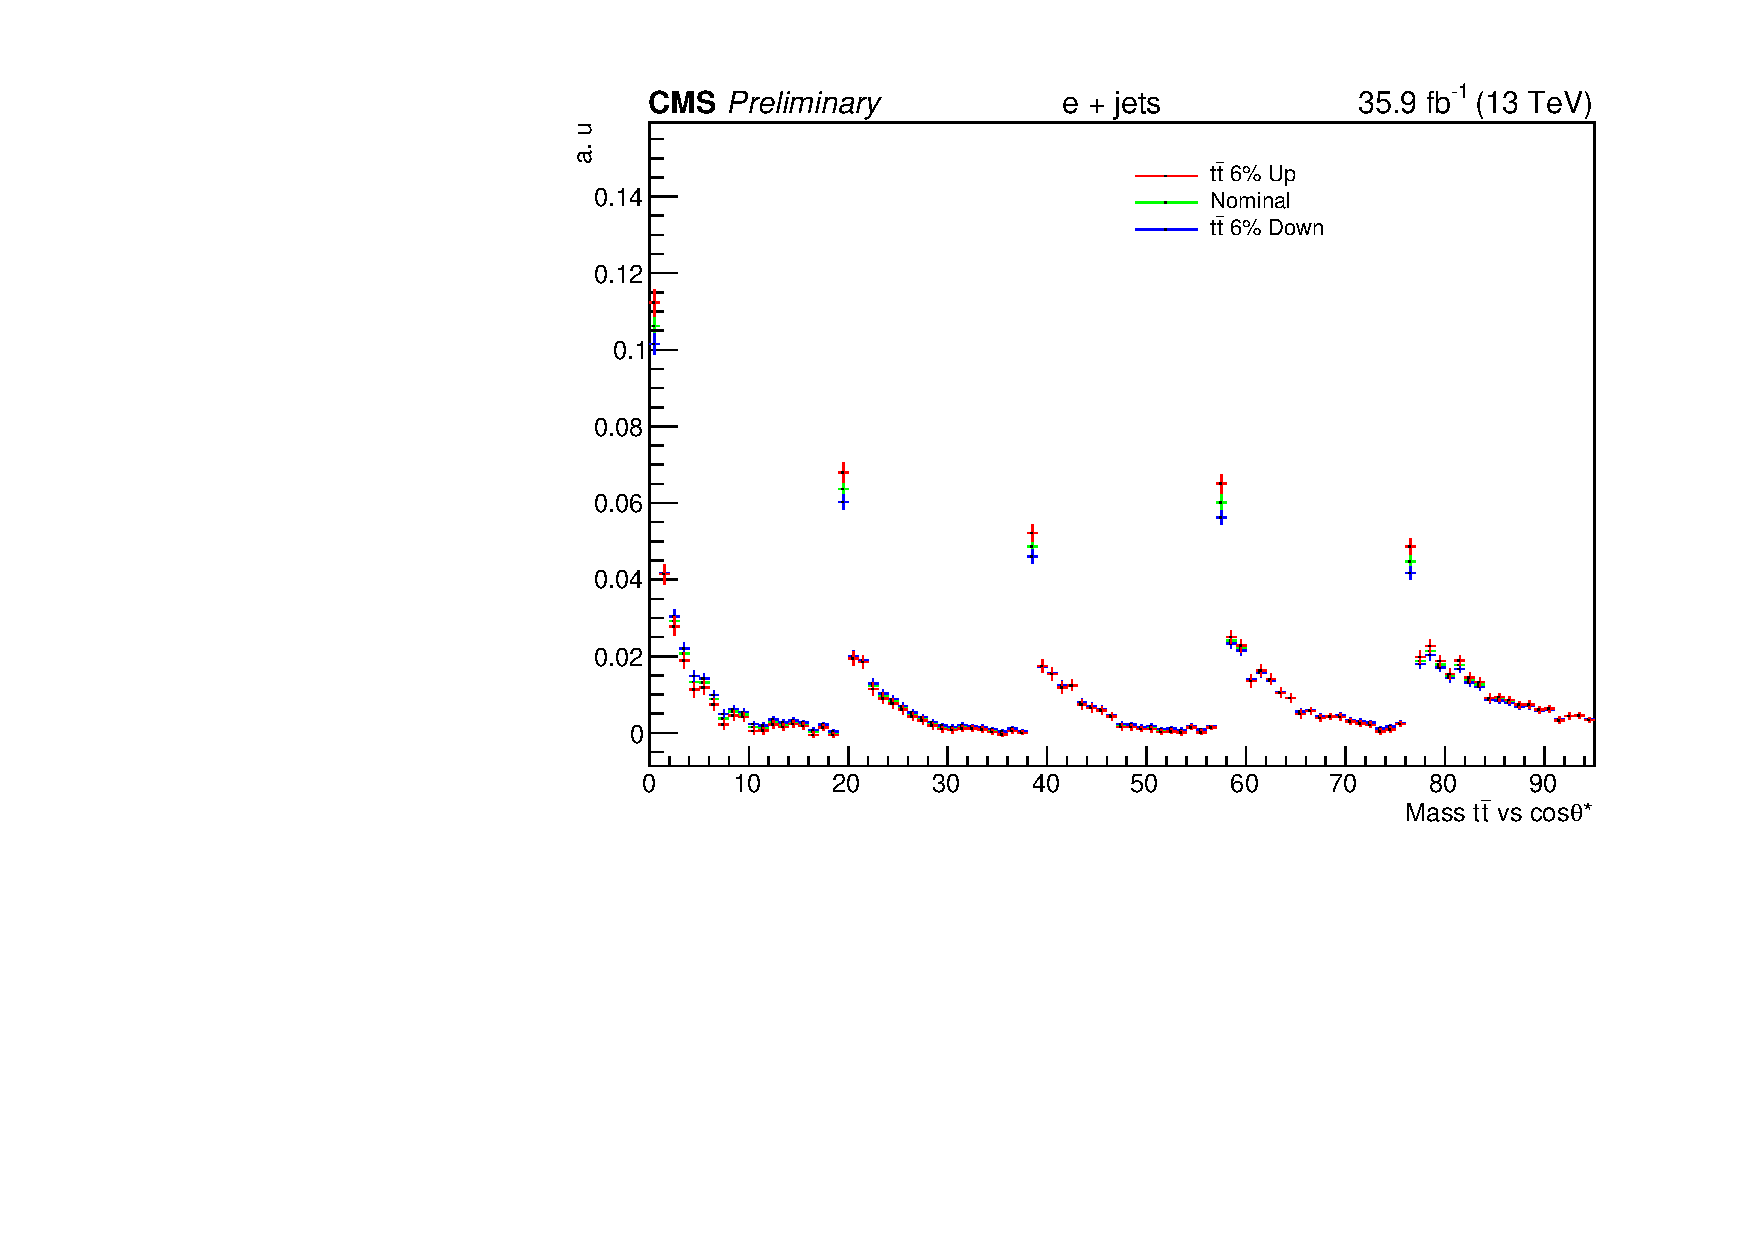
\includegraphics[scale=0.22]{fig/chapt7/qcd/qcd_e_ch/ttbar_m_cosine_ttsys_6perUpDn.pdf}\\
($\mathbf{m}$)\qquad\qquad&($\mathbf{n}$)\qquad\qquad&($\mathbf{o}$)\qquad\qquad&($\mathbf{p}$)\qquad\qquad\\
\\
\end{tabular}
\caption{(a) Shows cos$\theta$* and (b) mass of $t\overline{t}$ for the difference between Data and non-QCD MC in three isolation regions shown in table \ref{table:3Aiso_regions} for $\mu$ channel while (c) and (d) are the same kinematic distributions for electron channel. Distributions (e) and (f) show cos$\theta$* and mass of $t\overline{t}$ vs cos$\theta$* for the range  $0.15 \leq I_{rel}^{\mu}(\Delta\beta) < 0.43$ respectively for muon channel and (g) and (h) for electron channel with $0.0588 \leq I(\rho)$ for barrel and $0.0571 \leq I(\delta\rho)$ in endcap. Third row are the final data-driven multijet QCD distributions normalized to the area and used in fit for statistical evaluation. (i) and (j) are mass of $t\overline{t}$ and mass of $t\overline{t}$ vs cos$\theta$* distributions for $\mu$ channel and (k), (l) for electron channel. A 6\% statistical variation on $t\overline{t}$ is shown is last row for $\mu$ channel in (m), (n) and for electron channel in (o), (p).}\label{Fig:data_driven_qcd}
\end{figure}
%-------------------------------

%\renewcommand*{\thesection}{\thechapter.\arabic{section}}       % reset again to chaptnum.sectnum

\clearpage{\pagestyle{empty}\cleardoublepage}
